%-------------------------------------------------------------------------------
% * MSV Report Class Template and Documentation
\documentclass[twoside]{msvreport}
% - msvreport is an extension of the standard report class and passes
%   all options to report
% - default options are as in report class with exception of a4paper,
%   openright, and 11pt
% - msvcommon package is loaded and provides TUM color definitions,
%   logos, etc
%
%-------------------------------------------------------------------------------
% ** Options for msvreport (default options are marked (*))
% 1) boolean options for msvreport class:
%  | rmheads (*)    | use roman for headlines and contents                     |
%  | sfheads        | use sans-serif for headlines and contents                |
%  | chapterprefix  | print Chapter prefix in first chapter page               |
%  | bwchapters (*) | print chapter names in black                             |
%  | bluechapters   | print chapter names in blue                              |
%  | headrule       | print horizontal line in header                          |
%  | widetext (*)   | use a wide text body                                     |
%  | narrowtext     | use a narrow text body                                   |
%  | cmyk (*)       | use CMYK colors optimized for printing                   |
%  | print          | alias for cmyk                                           |
%  | rgb            | use RGB colors optimized for monitors                    |
%  | lores (*)      | use low-resolution TUM Banner                            |
%  | hires          | use high resolution TUM Banner                           |

%
% 2) Key/Value options for msvreport class
%  - coverstyle=(none|bw|banner|flags)
%    | none (*) | do not generate cover page                                               |
%    | color    | use color style for cover page                                           |
%    | bw       | use black/white style for cover page (eg for printing on colored covers) |
%    | banner   | use simple banner without flags for cover page (deprecated)              |
%    | flags    | use TUM flag banner for cover page (deprecated)                          |
%
%  - titlestyle=(flags|none|bw|banner)
%    same as coverstyle but for title page
%
%  - copyright=(none|cover|title)
%    | none (*) | do not print copyright notice           |
%    | cover    | print copyright notice after cover page |
%    | title    | print copyright notice after title page |
%
%
%-------------------------------------------------------------------------------
% ** MSV Font Package
% - Standard MSV Report fonts are Times for text and Computer Modern for maths
% - Use option timesmath to enable Times font also in math mode (only pdftex)
% - Do not use msvfonts package if you want to use your own fonts
% - Note that msvfonts loads amsmath package
%
\usepackage{msvfonts}
\usepackage{amssymb}
\usepackage{amsmath}
\usepackage{float}
\usepackage{subfig}
\usepackage[titletoc]{appendix}
\usepackage{siunitx}

\usepackage{listings}
\usepackage{soul,xcolor}\lstset{escapeinside={(*@}{@*)}}

% User defined Listing
\lstdefinestyle{DOS}
{
    backgroundcolor=\color{white},
    basicstyle=\scriptsize\color{black}\ttfamily
}


\usepackage{hyperref}
\usepackage{pdfpages}
\usepackage{rotating}
\usepackage{pdflscape}
\usepackage[acronym,nomain,nonumberlist,toc,shortcuts]{glossaries}


% Packages for Jonas Maas's Thesis Tikz block diagrams
\usepackage{tikz}
\usetikzlibrary{arrows.meta, calc}
\newcommand{\B}[1]{\boldsymbol{#1}}
\newcommand{\Bhat}[1]{\boldsymbol{\hat{#1}}}
\newcommand{\e}[1]{\emph{#1}}

\usepackage{caption}
%\usepackage{subcaption}
%\usepackage{capt-of}

%
% *** Options for msvfonts
% 1) boolean options for msvfonts package:
% | timestext (*) | use times font for text                                        |
% | fancytext     | use garamond font for text                                     |
% |             +-+                                                                |
% | cmrmath (*) | use computer modern font for text and operators in math-mode     |
% | timesmath   | use times font for text and operators in math mode               |
% |             |   WARNING: timesmath in LuaLaTeX uses unicode-math, which does   |
% |             |   not support the bm package. Use \symbfit and \symbf instead.   |
%
%
% -------------------------------------------------------------------------------
% ** Input Encoding
% - utf8x is recommended at MSV
% - Some comments on encoding can be found here:
%   https://groups.google.com/forum/?fromgroups=#!msg/comp.text.tex/4LC-xODb-LU/1Bd5UZOMNM4J
%
\ifxetexorluatex
  % XeTeX and LuaTeX support utf8 by default
\else
  % File encoding utf8x
  \usepackage{ucs}
  \usepackage[utf8x]{inputenc}
\fi
%
%--------------------------------------------------------------------------------
% ** Language Settings and Hyphenation Patterns
%
% Note: final argument to babel sets the main language
%
\ifxetex%
  \usepackage{polyglossia}
  \setmainlanguage{english}
  \setotherlanguage{german}
%  \setmainlanguage{german}
%  \setotherlanguage{english}
\else
  \usepackage[ngerman,english]{babel} 
\fi
%
%--------------------------------------------------------------------------------
% ** Custom Preamble
% - Start your custom preamble here
% - Use the space before \begin{document} to
%   - Load packages \usepackage{...}
%   - Define custom math operators (DeclareMathOperator)
% - Everything else (including newcommands) starts
%   below \begin{document}

% Here is a list of commonly used packages
% | amsmath   | Many useful tools for typesetting mathematics        |
% | amssymb   | Loads symbol fonts for mathematics, eg \mathbb       |
% | amsthm    | \newtheorem,\theoremstyle commands etc               |
% | thmtools  | Some advanced options for theorem customization      |
% | mathtools | Many useful tools for typesetting maths      |
% | bm        | Bold math (Warning: use only if bold fonts available |
% | algorithm | Tools to typeset algorithms                          |
% | booktabs  | Nice looking tables                                  |
% | enumerate | Enumerated lists                                     |
% | subfig    | Subfigures with common caption                       |
% | caption   | Control caption font                                 |
% | relsize   | Some useful relative font size commands              |
% | xspace    | Control white space after abbreviations              |
% | csquotes  | Quotations according to language selection           |

%-------------------------------------
% random.sty: for sans-serif math fonts
% use with:
%   \usepackage[greek,ngerman,english]{babel}
% does not work with 'timesmath' option in msvfonts
%

\setglossarystyle{long}
\renewcommand{\glsnamefont}[1]{\textbf{#1}}

\makeglossaries

\newacronym{MIMO}{MIMO}{Multiple Input Multiple Output}
\newacronym{GSM}{GSM}{Global System for Mobile communication}
\newacronym{LTE}{LTE}{Long Term Evolution}
\newacronym{RE}{RE}{Resource Elements}
\newacronym{FPGA}{FPGA}{Field Programmable Gate Array}
\newacronym{IEEE}{IEEE}{Institute of Electrical and Electronics Engineers}
\newacronym{PDSCH}{PDSCH}{Physical Downlink Shared Channel}
\newacronym{PDCCH}{PDCCH}{Physical Downlink Control Channel}
\newacronym{CRS}{CRS}{Cell Specific Reference Signal}
\newacronym{RF}{RF}{Radio Frequency}
\newacronym{PSS}{PSS}{Primary Synchronisation Signal}
\newacronym{SSS}{SSS}{Secondary Synchronisation Signal}
\newacronym{FDD}{FDD}{Frequency Division Duplexing}
\newacronym{TDD}{TDD}{Time Division Duplexing}
\newacronym{PCIe}{PCIe}{Peripheral Component Interconnect Express}
\newacronym{AFW}{AFW}{Application Framework}
\newacronym{BS}{BS}{Base Station}
\newacronym{UE}{UE}{User Equipment}
\newacronym{SNR}{SNR}{Signal to Noise Ratio}
\newacronym{BPSK}{BPSK}{Binary Phase Shift Keying}
\newacronym{QPSK}{QPSK}{Quadrature Phase Shift Keying}
\newacronym{PPS}{PPS}{Pulse Per Second}
\newacronym{OCXO}{OCXO}{Oven Controlled Crystal Oscillator}
\newacronym{AWGN}{AWGN}{Additive White Gaussian Noise}
\newacronym{OFDM}{OFDM}{Orthogonal Frequency Division Multiplexing}
\newacronym{PLL}{PLL}{Phase Locked Loop}
\newacronym{VCO}{VCO}{Voltage Controlled Oscillator}
\newacronym{TB}{TB}{Transport Block}
\newacronym{DMA}{DMA}{Direct Memory Access}
\newacronym{FIFO}{FIFO}{First In First Out}
\newacronym{CFO}{CFO}{Carrier Frequency Offset}
\newacronym{FFT}{FFT}{Fast Fourier Transform}
\newacronym{iFFT}{iFFT}{inverse Fast Fourier Transform}
\newacronym{DFT}{DFT}{Discrete Fourier transform}
\newacronym{INN}{INN}{Inverse Neural Network}
\newacronym{T2H}{T2H}{Target to Host}
\newacronym{H2T}{H2T}{Host to Target}
\newacronym{LUT}{LUT}{Look-up Table}
\newacronym{MCS}{MCS}{Modulation and Coding Scheme}
\newacronym{DCI}{DCI}{Downlink Control Indicator}
\newacronym{PRB}{PRB}{Physical Resource Block}
\newacronym{UL}{UL}{Uplink}
\newacronym{DL}{DL}{Downlink}
\newacronym{NI}{NI}{National Instruments}

\setlength\LTleft{0pt}
\setlength\LTright{0pt}
\setlength\glsdescwidth{0.8\hsize}

\begin{document}

%--------------------------------------------------------------------------------
% ** Custom Commands
% Put your \newcommand's here or \input them from a file
%
%
%--------------------------------------------------------------------------------
% ** Title and Author Information
%
\title{Experimental Evaluation of Machine Learning based Wireless Communication Algorithms}
\author{Karthik Sukumar}

\msvdoctype{Master Thesis}

\msvcovertext{
Supervisor: Prof. Wolfgang Utschick\\[1.5em]
Submission: Sep 07, 2020
}

%--------------------------------------------------------------------------------
% ** Title Page
%
\frontmatter
\maketitle
%
%--------------------------------------------------------------------------------
% ** Optional: Abstract
%
%\begin{abstract}
%    Put your abstract text here. 
%
%\end{abstract}

\listoffigures

\listoftables

%
%--------------------------------------------------------------------------------
% ** Table of Contents
%
\tableofcontents
%
%
%--------------------------------------------------------------------------------
%
% ** First Chapter

\mainmatter

\glsaddall
\printglossary[type=\acronymtype,title=Acronyms]

\chapter{Introduction}
\label{ch:intro}

Over the course of the internship many different parameters had to be determined and set up for the final demo. This chapters documents the results of all the experiments performed as well as the final demo of the working setup.

\section{Transmit Power Measurements}\label{GainDistortion}

A Rohde and Schwarz FSQ 8GHz spectrum analyser was used to capture the spurious emission at the output of the Spectrum analyser. The spectrum analyser had the following settings for this test.

\begin{table}[H]
    \begin{center}
        \begin{tabular}{|c|c|}
            \hline
            Parameter & Value \\ \hline
            RBW & 20kHz \\ \hline
            VBW & 50kHz \\ \hline
            SWP Time & 50ms  \\ 
            \hline
        \end{tabular}
    \end{center}
    \caption{Spectrum analyser settings for the transmit power tests}
    \label{}
\end{table}

An unmodulated test signal containing 2 sine tones each at 0.5 MHz and 1MHz was sent from the USRP transmitter with the measurement setup as shown below in the Figure \ref{fig:TxPwrSetup}. The 25W 20dB attenuator from spinner (Pt No: 36234) was used to protect the input of the spectrum analyser from high power.

%\begin{figure}[!htb]
%    \centering
%    \includegraphics[width=7cm]{../ReportImages/TxPwrSetup.png}
%    \caption{Setup for measuring the transmit power}%
%    \label{fig:TxPwrSetup}%
%\end{figure}

The results in Figure \ref{fig:GainDistortion} and Table \ref{tab:LinkBudgetMeas} show that any gain setting above 60 results in out of band emissions. Hence the maximum setting was chosen, which did not introduce any out of band emissions, namely Tx Gain setting of 60 which corresponds to -25dBm.

\begin{table}[H]
\centering
\begin{tabular}{|c|c|c|c|c|}
\hline
\begin{tabular}[c]{@{}c@{}}Tx Gain\\ Setting\\ USRP\end{tabular} & \begin{tabular}[c]{@{}c@{}}Attenuator\\ (dBm)\end{tabular} & \begin{tabular}[c]{@{}c@{}}Tx Power\\ Measured\\ (dBm)\end{tabular} & \begin{tabular}[c]{@{}c@{}}Tx Power\\ Actual\\ (dBm)\end{tabular} & \begin{tabular}[c]{@{}c@{}}Distortion\\ observed\end{tabular} \\ \hline
\multicolumn{1}{|c|}{35}                                         & \multicolumn{1}{c|}{20}                                    & \multicolumn{1}{c|}{-70.18}                                         & \multicolumn{1}{c|}{-50.18}                                       & \multicolumn{1}{c|}{No}                                       \\ \hline
\multicolumn{1}{|c|}{40}                                         & \multicolumn{1}{c|}{20}                                    & \multicolumn{1}{c|}{-64.95}                                         & \multicolumn{1}{c|}{-44.95}                                       & \multicolumn{1}{c|}{No}                                       \\ \hline
\multicolumn{1}{|c|}{45}                                         & \multicolumn{1}{c|}{20}                                    & \multicolumn{1}{c|}{-60.01}                                         & \multicolumn{1}{c|}{-40.01}                                       & \multicolumn{1}{c|}{No}                                       \\ \hline
\multicolumn{1}{|c|}{50}                                         & \multicolumn{1}{c|}{20}                                    & \multicolumn{1}{c|}{-54.9}                                          & \multicolumn{1}{c|}{-34.9}                                        & \multicolumn{1}{c|}{No}                                       \\ \hline
\multicolumn{1}{|c|}{55}                                         & \multicolumn{1}{c|}{20}                                    & \multicolumn{1}{c|}{-50.05}                                         & \multicolumn{1}{c|}{-30.05}                                       & \multicolumn{1}{c|}{No}                                       \\ \hline
\multicolumn{1}{|c|}{60}                                         & \multicolumn{1}{c|}{20}                                    & \multicolumn{1}{c|}{-44.99}                                         & \multicolumn{1}{c|}{-24.99}                                       & \multicolumn{1}{c|}{No}                                       \\ \hline
\multicolumn{1}{|c|}{65}                                         & \multicolumn{1}{c|}{20}                                    & \multicolumn{1}{c|}{-39.96}                                         & \multicolumn{1}{c|}{-19.96}                                       & \multicolumn{1}{c|}{Yes}                                      \\ \hline
\multicolumn{1}{|c|}{70}                                         & \multicolumn{1}{c|}{20}                                    & \multicolumn{1}{c|}{-34.77}                                         & \multicolumn{1}{c|}{-14.77}                                       & \multicolumn{1}{c|}{Yes}                                      \\ \hline
\multicolumn{1}{|c|}{75}                                         & \multicolumn{1}{c|}{20}                                    & \multicolumn{1}{c|}{-29.9}                                          & \multicolumn{1}{c|}{-9.9}                                         & \multicolumn{1}{c|}{Yes}                                      \\ \hline
\multicolumn{1}{|c|}{80}                                         & \multicolumn{1}{c|}{20}                                    & \multicolumn{1}{c|}{-24.9}                                          & \multicolumn{1}{c|}{-4.9}                                         & \multicolumn{1}{c|}{Yes}                                      \\ \hline
\end{tabular}
\caption{Distortion Values}
\label{tab:my-table}
\end{table}

\section{Path Loss Measurements}\label{PathLossMeasurements}

The measurements were performed in the Nokia car park entrance as shown below in Figure \ref{fig:NokiaCarpark}. The free space path loss experiments were performed by setting the transmit power to -25dBm and measuring the received power at Line of Sight(LoS) locations which were 4,6,8 and 10m apart.

\begin{table}[H]
\centering
\begin{tabular}{ccccccc}
\hline
\multicolumn{1}{|c|}{\begin{tabular}[c]{@{}c@{}}Range \\ (m)\end{tabular}} & \multicolumn{1}{c|}{\begin{tabular}[c]{@{}c@{}}Tx Pwr\\ (dBm)\end{tabular}} & \multicolumn{1}{c|}{\begin{tabular}[c]{@{}c@{}}Antenna \\ Gain (dBi)\end{tabular}} & \multicolumn{1}{c|}{\begin{tabular}[c]{@{}c@{}}Calculated\\ Path Loss(dBm)\end{tabular}} & \multicolumn{1}{c|}{\begin{tabular}[c]{@{}c@{}}Expected Rx \\ Pwr(dBm)\end{tabular}} & \multicolumn{1}{c|}{\begin{tabular}[c]{@{}c@{}}Measured\\ (dBm)\end{tabular}} & \multicolumn{1}{c|}{\begin{tabular}[c]{@{}c@{}}Delta\\ (dBm)\end{tabular}} \\ \hline
\multicolumn{1}{|c|}{4}                                                    & \multicolumn{1}{c|}{-25}                                                    & \multicolumn{1}{c|}{4.0}                                                           & \multicolumn{1}{c|}{49.0}                                                                & \multicolumn{1}{c|}{-66.0}                                                           & \multicolumn{1}{c|}{-69.8}                                                    & \multicolumn{1}{c|}{-3.8}                                                  \\ \hline
\multicolumn{1}{|c|}{6}                                                    & \multicolumn{1}{c|}{-25}                                                    & \multicolumn{1}{c|}{4.0}                                                           & \multicolumn{1}{c|}{53.0}                                                                & \multicolumn{1}{c|}{-70.0}                                                           & \multicolumn{1}{c|}{-74.5}                                                    & \multicolumn{1}{c|}{-4.5}                                                  \\ \hline
\multicolumn{1}{|c|}{8}                                                    & \multicolumn{1}{c|}{-25}                                                    & \multicolumn{1}{c|}{4.0}                                                           & \multicolumn{1}{c|}{55.8}                                                                & \multicolumn{1}{c|}{-72.8}                                                           & \multicolumn{1}{c|}{-75.8}                                                    & \multicolumn{1}{c|}{-3.0}                                                  \\ \hline
    \multicolumn{1}{|c|}{10}                                                   & \multicolumn{1}{c|}{-25}                                                    & \multicolumn{1}{c|}{4.0}                                                           & \multicolumn{1}{c|}{58.0}                                                                & \multicolumn{1}{c|}{-75.0}                                                           & \multicolumn{1}{c|}{-77.3}                                                    & \multicolumn{1}{c|}{-2.3}                                                  \\ \hline
                                                                           &                                                                             &                                                                                    &                                                                                          &                                                                                      &                                                                               &                                                                            \\ \cline{6-7} 
                                                                           &                                                                             &                                                                                    &                                                                                          & \multicolumn{1}{c|}{}                                                                & \multicolumn{1}{c|}{Mean}                                                     & \multicolumn{1}{c|}{-3.4}                                                  \\ \cline{6-7} 
\end{tabular}
\caption{Path Loss Measurements}
\label{tab:LinkBudgetMeas}
\end{table}

\section{Transmit and Receive Loopback}

This test was performed to test and identify the transmitter and receiver system response without the air interface. The system should ideally return a flat response across all the subcarriers with a magnitude of 0dBm. But due to cable and insertion losses the response is lower than 0dBm. Figure \ref{fig:TxRxLoopback} shows the mean value of the magnitude in dB over the frequency is -2.36dBm which corresponds approximately to the loss figure obtained from Section \ref{PathLossMeasurements}. The other losses could be attributed to insertion losses when the antenna is plugged in on both ends.

For this experiment the transmit power was -25dBm with the center frequency 2.6GHz and the LTE Frame described in Section \ref{LTEFrame} was transmitted. The transmitter was connected to the receiver with the help of a 1.5m long 50 \si{\ohm} coaxial cable.

\section{Radar Calibration}

An object was placed in the horizontal axis of the radar sensor at a distance of 10m from the radar sensor. Markings were laid out on the road as shown in the figure \ref{fig:RadarCenter} and the reading was compared to the data processed by the radar sensor which was 10.1m still within the accuracy of the radar sensor.

\section{Hardware Performance}

\subsection{USRP Sampling Rate}\label{ssec:USRPSamplingRate}
The USRP Software defined radio is very convenient for prototyping. There are although some drawbacks with using the drivers in MATLAB. Experiments with the full LTE bandwidth of 20MHz resulted in consistently dropped frames and consequently led to unreliable channel estimation data. On further investigation it was found that the MATLAB drivers were single threaded and could not allocate sufficient buffers in the kernel to support the higher sampling rates of 15.36MSps and 30.72MSps. Therefore a 7.68MSps was chosen which corresponds to a 5MHz LTE bandwidth as this worked the most reliabily with the current available hardware. Alternatives to MATLAB to USRP interface is described in Section \ref{ssec:GNURadio}.

\subsection{Max Frame Rate for Demo}
Real time processing of channel estimation is an especially demanding operation for a general purpose compute platform. The performance was better on a more powerful intel i7 compared to an intel i5 processor.

It was also found that the USRP drivers worked more reliably on a linux platform than on a windows platform i.e: for a given USRP sampling rate the frame drops were seldom observed on the linux platform. Table \ref{tab:OSComp} is a comparison of a standalone channel estimation application running on MATLAB on 2 devices and the approximate frame rates that could be achieved. The frame rate performance does degrade upon running other compute intensive programs simultaneously.

\begin{table}[H]
\centering
\begin{tabular}{ccc}
\hline
\multicolumn{1}{|c|}{}                & \multicolumn{1}{c|}{OS}         & \multicolumn{1}{c|}{\begin{tabular}[c]{@{}c@{}}Update Rate\\ Frames/s\end{tabular}} \\ \hline
\multicolumn{1}{|c|}{Nokia Laptop}    & \multicolumn{1}{c|}{Windows 10} & \multicolumn{1}{c|}{1-2}                                                                 \\ \hline
\multicolumn{1}{|c|}{Personal Laptop} & \multicolumn{1}{c|}{Linux} & \multicolumn{1}{c|}{8-10}                                                                \\ \hline
\end{tabular}
\caption{Comparison on different operating systems}
\label{tab:OSComp}
\end{table}


\section{Demo}
The demo took place in the carpark entrance of the Nokia Munich site in St.Martin Straße as shown in Figure \ref{fig:NokiaCarpark}. The setup for the final demo is shown in the Figure \ref{fig:TestSetup} below. The LTE frame was transmitted by a laptop running on a Linux OS continously transmitting LTE frames. The laptop across the street was connected to the USRP, which receives and decodes the LTE frames. The radar sensor is also attached to this computer to get the range and angle data. The laptops were placed approximately 15m apart on opposite sides of the carpark entry ramp.

Shown below in Figure \ref{fig:TestSetupLegend} is a legend of what is seen as a part of the demo video and the subsequent figures that follow this. The first figure on top shows position of the object w.r.t the Radar transceiver. The 2nd figure displays the 2D channel estimate in both the time axis as well as the frequency axis (subcarriers). The third figure below the 2D grid shows the trend of the first, middle and the last subcarrier namely 1,150 and 300 subcarriers. The magnitude for both the plots is in dBm and the x axis on the figure at the bottom represents the symbols captured. This is 20 Symbols per frame, this is the compressed information picking only every 7th symbol in the frame of 140 symbols.

Figures \ref{fig:DemoBefore} - \ref{fig:DemoAfter} show the screen captures of an object passing through the LoS channel. The Figures \ref{fig:DemoBefore}, \ref{fig:DemoDuring2} and \ref{fig:DemoAfter} show the state of the channel before, during and after the object has passed. The object passed by around 9m and this is shown in Figure \ref{fig:DemoDuring2}. The channel trend shows that the channel is severely attenuated when the object obstructs the channel. This can also be infered from Figure \ref{fig:DemoBefore} and Figure \ref{fig:DemoAfter} where the channel returns to normal.

The full video of the demo can be viewed here \cite{demoVideo}.

\chapter{System Model}
\label{ch:sysmodel}

As mentioned in Chapter \ref{ch:intro}, the goal of this thesis is to obtain measurement data from the MIMO setup. This collected experimental data will be applied to the machine learning model which has been developed in parallel with this thesis. In this chapter the relevant fundamentals of the LTE standard, which will be used as a basis for our experiments are described on a high level.

%\par
%
%In the following sections we would discuss the LTE frame structure and the relevant signalsthat are required for the collection of the data. The release of the LTE standard being used here is the Release 10.

\section{LTE}\label{sec:LTEProc}

LTE stands of Long Term Evolution and is a successor standard to UMTS. LTE is a multicarrier approach for multiple access which uses Orthogonal Frequency-Division Multiple Access (OFDMA) in the physical layer. OFDM uses multiple carriers (known as sub carriers) spaced equally apart and can transmit independent data streams on each sub carrier \cite{rohling}.

\par

Hence an LTE frame is commonly represented as a 2D time frequency grid, where the vertical axis represents the sub-carriers(Frequency) and the horizontal axis represents time. LTE also comes in 2 flavours Frequency Division Duplexing (FDD) and Time Division Duplexing (TDD). In this thesis the focus will be on FDD systems, which use seperate frequency bands, for uplink and for downlink data respectively. The advantage of an FDD system is that the uplink and downlink transmittion can happen simultaneously.

LTE has a certain predefined signal symbol structure according to the standard \cite{3gpp36211}. In the following sections the frame structure and the different symbols in the LTE Frame shall be introduced.

\section{LTE Waveform Processing}\label{sec:LTE Waveform Processing}
LTE stands of Long Term Evolution and is a successor standard to UMTS. LTE is a multicarrier approach for multiple access which uses Orthogonal Frequency-Division Multiple Access (OFDMA) in the physical layer. OFDM uses multiple carriers (known as sub carriers) spaced equally apart in frequency and can transmit independent data streams on each sub carrier \cite{rohling}. LTE also comes in 2 flavours Frequency Division Duplexing (FDD) and Time Division Duplexing (TDD). In this report the focus will be on FDD systems, which uses seperate frequency bands for uplink and for downlink data so that the uplink and downlink data can be transmitted simultaneously.

LTE was chosen as a standard to use for the communication system given the integrated support of simulation environments like MATLAB and Simulink and that it is currently widespread in the telecommunications industry.

\subsection{Transmission} \label{ssec:Transmission}

A dual antenna transmitter using a USRP software defined radio as mentioned in \ref{sec:USRP} is used for the interface. A modified version of the LTE Application framework with MIMO 2x2 extension is used to log the data and run with different parameters. The transmitter USRP is connected to a Host PC using a 4-lane PCIe connection. This is necessary for the high data throughput exchanged between the host and the devices.

LTE has a standardized frame structure which is commonly represented as a 2D time frequency grid, where the vertical axis represents the sub-carriers and the horizontal axis represents time. LTE also uses a predefined signalling structure according to the standard \cite{3gpp36211}. In the following sections the frame structure and the symbols relavent to channel estimation shall be introduced.

\subsubsection{LTE Frame} \label{LTEFrame}

A single frame is 10ms long and consists of 10 smaller units called subframe, each 1ms long. A symbol is the smallest unit of time for an LTE system and one subframe has 14 such symbols each approximately 66.7us long. Scheduling is normally done on a subframe basis for both uplink and downlink communication.

LTE's time frequency grid contains many different signals each performing specific funtionality like broadcasting, control channel information, data transfer, among other functions.

For the puprpose of channel estmation, the most important signals are Primary Synchronisation Signal(PSS), Secondary Synchronisation Signal (SSS) and Cell Specific Reference Signal (CRS) which are described in detail in the subsequent sections.

\subsubsection {Primary Synchronisation Signal (PSS)} \label{sssec:PSS}
        OFDM is extremely time and frequency sensitive, hence it is very important to know the exact start of every frame. The PSS helps to achieve the synchronisation of the frame by using a specific sequence called the Zadoff-Chu sequence \cite{3gpp36211}.
        The Zadoff-Chu sequence has the property of constant amplitude zero autocorrelation waveform (CAZAC sequences) that cyclically shifted versions of the waveform are orthogonal to each other. The sequence is described in Equation \ref{eq:ZCSeq} where {\em u}  can be 25,29 or 34 depending on the cell ID.
        The PSS is broadcast twice every radio frame and the symbols are identical each time.

\begin{equation} \label{eq:ZCSeq}
        d_u(n) =
        \begin{cases}
            \mathrm{e}^{-j\frac{\pi un(n+1)}{63}}       & \quad n=0,1,...,30\\
            \mathrm{e}^{-j\frac{\pi un(n+1)(n+2)}{63}} & \quad n=31,32,...,61
        \end{cases}
\end{equation}

\subsubsection{Secondary Synchronisation Signal (SSS)} \label{sssec:SSS}
        The SSS is a 62 bit pseudo random sequence \cite{3gpp36211}. It is broadcast twice in a frame once in subframe 0 and once in subframe 5, one symbol before the PSS. The 2 sequences of transmission in a frame are different so that the UE can identify which position in the frame the synchronisation happens.

\subsubsection{Cell Specific Reference Signal (CRS)} \label{sssec:CRS}
        As mentioned in Chapter \ref{ch:intro} the channel needs to be estimated in order to reverse the channel propogation effects. With the help of CRS the channel can be estimated by placing equally spaced reference symbols along every 6 subcarriers starting from subcarrier 2 on symbols 1, 8, 15, etc... and every 6 subcarriers starting from subcarrier 5 on symbols 5, 12, 19, etc...\cite{3gpp36211}. The signals received by the UE and the channel effects are inferred based on amplitude damping and phase shift. Placing the signals in the above defined spacing gives the best coverage to interpolate over in time and frequency.

        The signals to be placed on the grid are decided by the Equation \ref{eq:CRS} as shown below, with the parameters defined in Table \ref{tab:CRSParam} \cite{3gpp36211}.
        \begin{equation} \label{eq:CRS}
            r_{l,n_s}(m) = \frac{1}{\sqrt{2}}(1-2{\cdot}c(2m)) + j\frac{1}{\sqrt{2}}(1-2{\cdot}c(2m+1)),\ m=0,1,...,2N_{RB}^{max,DL}-1
        \end{equation}

        \begin{table}[H]
            \begin{center}
                \begin{tabular}{|l|l|}
                    \hline
                    Parameter& Description\\ \hline
                    $c(m)$& Pseudo Random Sequence defined in \cite{3gpp36211}\\ \hline
                    $N_{RB}^{max,DL}$& Maximum number of Downlink resources blocks\\ \hline
                    $n_s$& Slot number in the frame\\ \hline
                    $l$& OFDM Symbol number in the frame\\
                    \hline
                \end{tabular}
                \caption{Parameter definitions for evaluating CRS Symbols}
                \label{tab:CRSParam}
            \end{center}
        \end{table}

%\subsubsection{PDCCH}

%//TODO add the time domain and spectrum figure

\subsubsection{Final Waveform}
All the signals mentioned in Section \ref{LTEFrame} are generated in Labview using the LTE Application Framework Software and arranged in a 2D grid of frequency and time as shown below in Figure \ref{fig:RBSignals}. The CRS are placed every 6 subcarriers in the frequency domain and every 3 or 4 time symbols apart, according to the position on the grid. Where as the PSS and SSS only repeat every 5 subframes.

\begin{figure}[H]
    \begin{center}
        %\includegraphics[wisdth=\linewidth]{../ReportImages/RB_legend.jpg}
        \caption{Resource Block Grid for 2 sub frames}
        \label{fig:RBSignals}
    \end{center}
\end{figure}

One of the disadvantages of using OFDM in the physical layer is the high peak to average power ratio (PAPR) of the signal. High PAPR translates to high fidelity requirements of power amplifiers on the transmitter side. It also induces non-linear distortions to the signal \cite{rohling}. To ensure that the PAPR of the signal is as low as it can be, random QPSK symbols are transmitted on the unused slots instead of 0s.

\subsection{Reception}

For the LTE receiver processing a USRP captures in bursts and streams the data to a laptop connected via a USB interface. The signals are processed by a custom MATLAB application which performs the necessary steps to decode the LTE Frames, estimate the channel and display the information as a 3D surface. For the case of the demo the data was processed as soon as they were received from the USRP and the channel estimate was displayed in realtime. The data can alternatively be logged for offline postprocessing to get better granularity as intermittent processing delays dont appear.

Once enough samples have been captured (usually 2 or more Frames) the data can be processed in the following steps.


\subsubsection{Carrier Offset Estimation and Correction}
OFDM is extremely senstive to frequency shifts in the received signal. In the case that the receiver or transmitter center frequency clock was not accurate enough, the frequency shift needs to be estimated and corrected. This is the very first step before processing the baseband waveform.

%TODO

\subsubsection{Frame synchronisation}
As mentioned in Section \ref{LTEFrame} the synchronisation is a very important part of knowing where the LTE frame begins. This is done by correlating the received signal with the known Zadoff Chu Sequence and to look for the peak. Figure \ref{fig:PSSCorr} shows an example correlation of a Zadoff Chu sequence and a received signal containing 307200 samples in total amounting to 2 frames of a 10MHz Bandwidth LTE signal. 4 peaks are to be expected here as there are 2 frames, each containing 2 PSS sequences.

\begin{figure}[H]
    \begin{center}
        %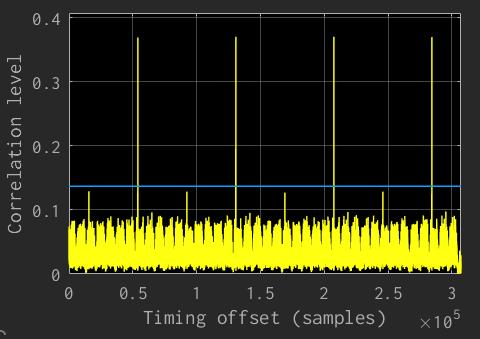
\includegraphics[width=9cm]{../ReportImages/PSSCorrelation.jpg}
        \caption{PSS Correlation}
        \label{fig:PSSCorr}
    \end{center}
\end{figure}

\subsubsection{Channel Estimation}

Once the frame has been demodulated and the 2D OFDM grid has been obtained, the channel can be estimated based on the original pilot symbols structure known to the receiver, hence the phase and amplitude of the particular sub carrier can be obtained. A 2D wiener filter is applied in both the time and frequency axis to interpolate the channel estimate. More explained in the Chapter \ref{ch:ChEst}.

%TODO

\subsection{Antenna}
The analog time domain signal is transmitted from the USRP (Section \ref{sec:USRP}) over the air using a Triband antenna. For the setup an omni directional Antenna from TODO capable of transmitting and receiving around frequencies of 144, 400 or 1200 MHz. This antenna shown in Figure \ref{fig:USRPAnt} was used as the transmit and the receive antenna for the demo setup.

\begin{figure}[H]
    \begin{center}
        %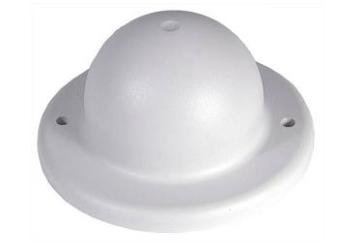
\includegraphics[width=7cm]{../ReportImages/HuberAntenna.png}
        \caption{Narrowband Omnidirectional Antenna used for transmitting and receiving the LTE Signals}
        \label{fig:USRPAnt}
    \end{center}
\end{figure}

\chapter{Channel Estimation}\label{ch:ChEst}

LTE was chosen as the standard to use here as it is very mature and has readily available MATLAB/Labview based implementation. In the case of this thesis the aim is not to reinvent standard by redesigning pilot symbol placements, instead existing standards were used in order to collect experimental data. This reduces design time and focusses on the issue at hand which is channel estimation data of a MIMO Channel.

\section{OFDM}\label{sec:OFDM}
LTE is based on OFDMA in the physical layer which is a multi carrier communication scheme \cite{FazelKaiser}. As the name suggests OFDM uses orthogonal sub carriers from an orthonormal system to form the basis for independent data streams. For band limited transmission systems with finite access time per channel use the dimension of the parallel data stream is given by the Equation \ref{eq:BandLim}  \cite{UtschickOFDM}.

        \begin{equation} \label{eq:BandLim}
            N = BT
        \end{equation}

        \begin{table}[H]
            \begin{center}
                \begin{tabular}{|c|l|}
                    \hline
                    Parameter& Description\\ \hline
                    $N$& Dimension of system \\ \hline
                    $B$& Signal Bandwidth \\ \hline
                    $T$& Channel access time \\
                    \hline
                \end{tabular}
                \caption{Parallel data streams parameter description}
                \label{tab:BandLimTrans}
            \end{center}
        \end{table}

The orthonormal basis function can be mathematically modelled as the Equation \ref{eq:OFDM} \cite{UtschickOFDM}.

        \begin{equation} \label{eq:OFDM}
            \begin{split}
                \psi_{b,q} = p_{T_{b}}(t)exp(j2{\pi}q{\frac{t}{T}}) \\
                p_{T_{b}}(t) = \left\{
                    \begin{matrix}
                        1; & t \in T_b \\
                        0; & otherwise \\
                    \end{matrix}\right.
            \end{split}
        \end{equation}

        \begin{table}[H]
            \begin{center}
                \begin{tabular}{|c|l|}
                    \hline
                    Parameter& Description\\ \hline
                    $\psi_{b,q}$& normalized orthogonal basis functions\\ \hline
                    $b$& channel access slot\\ \hline
                    $q$& sub carrier index\\ \hline
                    $T$& channel access time \\ \hline
                    $T_{b}$& $ bT \leq t < (b + 1)T \subset \mathbb{R}$ \\ \hline
                \end{tabular}
                \caption{}
                \label{tab:OFDMParam}
            \end{center}
        \end{table}


        The transmitted data can hence be modelled as the following
        \begin{equation} \label{eq:TxDataMath}
            x_b(t) = \sum_{q=0}^{N-1}\underbrace{X_{b,q}}_\text{data} \psi_{b,q}(t)
        \end{equation}

        For a given ideal AWGN Channel, where there is no delay spread or multipath propogation, the corresponding received data is modelled as
        \begin{equation} \label{eq:RxDataMathIdeal}
            y_b(t) = \sum_{q=0}^{N-1}x_b(t) \psi_{b,q}(t) +\eta_b(t)
        \end{equation}
        where $\eta_b(t)$ is the additive noise

        The demodulation is based on the same set of orthonormal basis vectors as that of the transmitter, hence we have
        \begin{equation}
            \begin{aligned}\label{eq:InnerProductRxIdeal}
                \hat{x}_{b,q} = \langle y,\psi_{b,q}(t)\rangle + \langle\eta_{b},\psi_{b,q}(t)\rangle = x_{b,q}(t) + \eta_{b,q} & & & \forall q = 1,...,N \\
            \end{aligned}
        \end{equation}

        In the case of a channel with delay spread (also referred to as multipath propogations) we model it as the following
        \begin{equation} \label{eq:DelaySpread}
            \begin{split}
                h(t) = \sum_{l=0}^{L-1}h_l\delta{(t-l\frac{T}{N})} \\ 
            \end{split}
        \end{equation}
        where $h$ is the time domain channel taps. The term $h_lx_{b,q}\psi_q(t-l\frac{T}{N}-bT)$ leads to interference between adjacent channels $T_{b-1},T_{b},T_{b+1}$, etc. This has be avoided to have faithful reproduction of transmitted data on the receiver end.

\subsection{Cyclic Prefix}\label{ssec:CP}

As a result of Equation \ref{eq:DelaySpread} we have to compensate for the interference of the symbols of the $b_{th}$ channel with the other channels. A simple solution to this interference is a Cyclic prefix. As the name suggests it is a cyclic addition of the signal at the transmitter end, which means copying the beginning of the signal and adding it to the end. To this end $T = T + T_p$, where $T_p$ is the duration of the cyclic prefix. In the LTE standard the cyclic prefix lengths are predefined based the normal or extended mode \cite{3gpp36211}

\begin{equation}
    \begin{split}
        \psi_{b,q}(t) = p_{T_b}(t)exp\left( j2\pi{q}\frac{t}{T} \right) \\
        \text{where} \; \psi_{b,q} \in T_b = [-T_p + bT_s , bT_s + T [
    \end{split}
\end{equation}

This is illustrated in the Figure \ref{fig:CPIlls}

\begin{figure}[H]
    \begin{center}
        \includegraphics[width=\linewidth]{images/CP_illustration.png}
        \caption{Cyclic prefix addition \cite{UtschickOFDM}}
        \label{fig:CPIlls}
    \end{center}
\end{figure}

On the receiver end

\begin{equation}
    y_{b,n} = \sum_{l=1}^{L-1}h_l\delta_{n-l} \ast \sum_{l=-Np}^{N-1}x_{b,k}\delta_{n-k} = \sum_{l=1}^{L-1}\sum_{k=-Np}^{N-1}h_lx_{b,k}\delta_{n-l-k}
\end{equation}

subject to $L-1 \leq N_p$ ,where $N_p$ is the number of samples of the cyclic prefix

\begin{equation}
    \begin{aligned}
        y_{b,n} & = \sum_{l=1}^{L-1}h_lx_{b,n-l} = \sum_{l=1}^{L-1}h_lx_{b,mod_N(n-l)}, & & n,q \in 0,\cdots ,N-1
        \\
        y_{b,n} & = h_n \circ x_{b,n} \Leftrightarrow \frac{1}{N}Y_{b,q} = H_qX_{b,q}, & & n,q \in 0,\cdots,N-1
    \end{aligned}
\end{equation}

\begin{equation}\label{eq:MatrixConvCP}
    \begin{bmatrix}
        y_{b,-2}
        \\ y_{b,-1}
        \\ y_{b,0}
        \\ y_{b,1}
        \\ y_{b,2}
        \\ y_{b,3}
    \end{bmatrix}
    =
    \begin{bmatrix}
        h_0 &  &  &  &  & \\ 
        h_1 & h_0 &  &  &  & \\ 
        h_2 & h_1 & h_0 &  &  & \\ 
        & h_2 & h_1 & h_0 &  &  \\ 
        & & h_2 & h_1 & h_0 &  \\ 
        & & & h_2 & h_1 & h_0
    \end{bmatrix}
    \begin{bmatrix}
        x_{b,-2}
        \\ x_{b,-1}
        \\ x_{b,0}
        \\ x_{b,1}
        \\ x_{b,2}
        \\ x_{b,3}
    \end{bmatrix}
    +
    \begin{bmatrix}
        h_2 & h_1 & & & & \\ 
        &  h_2 &  &  &  & \\ 
        &  &  &  &  & \\ 
        &  &  &  &  & \\ 
        &  &  &  &  & \\ 
        &  &  &  &  & 
    \end{bmatrix}
    \begin{bmatrix}
        x_{b-1,2} \\ 
        x_{b-1,3} \\ 
        0 \\
        0 \\ 
        0 \\ 
        0 
    \end{bmatrix}
    +
    \begin{bmatrix}
        \eta_{b,-2}\\ 
        \eta_{b,-1}\\ 
        \eta_{b,0}\\ 
        \eta_{b,1}\\ 
        \eta_{b,2}\\ 
        \eta_{b,3}
    \end{bmatrix}
\end{equation}

With a cyclic prefix chosen such that $x_{b,-n} = x_{b,N-n}, n \leq N_p $, then $x_{b,-1}$ and $x_{b,-2}$ can be deleted and equation \ref{eq:MatrixConvCP} can be rearranged as the following

\begin{equation}\label{eq:MatrixConvCPSimpl}
    \begin{bmatrix}
        y_{b,0}
        \\ y_{b,1}
        \\ y_{b,2}
        \\ y_{b,3}
    \end{bmatrix}
    = 
    \begin{bmatrix}
        h_0 &  &h_2 & h_1 \\ 
        h_1 & h_0 & & h_2 \\ 
        h_2 & h_1 & h_0 & \\ 
        & h_2 & h_1 & h_0
    \end{bmatrix}
    \begin{bmatrix}
        x_{b,0}
        \\ x_{b,1}
        \\ x_{b,2}
        \\ x_{b,3}
    \end{bmatrix}
    +
    \begin{bmatrix}
        \eta_{b,0}\\ 
        \eta_{b,1}\\ 
        \eta_{b,2}\\ 
        \eta_{b,3}
    \end{bmatrix}
\end{equation}

Taking the DFT of equation \ref{eq:MatrixConvCPSimpl} gives 

\begin{equation}\label{eq:DFTCP}
    y_b = \hat{H}x_b + \eta_{b} \Leftrightarrow Y_b = \frac{1}{N}F\hat{H}F^HX_b + F\eta_{b}
\end{equation}

Where $F$ is the fourier matrix. Since $\hat{H}$ is a circulant matrix (also a convolutional matrix) it can be broken down as equation \ref{eq:CircMtxExp} \cite{CircMatrixStanford}. The eigenvalues of the circulant matrix are the fourier transformed coefficients of the first column while the eigenvectors are the columns of the inverse fourier transform matrix. Equation \ref{eq:CircMtxExp} presents a eigenvector decomposition of matrix $\hat{H}$ where $F^H$ is the inverse DFT matrix and $\Lambda$ is the diagonal matrix with entries being the fourier transform terms of the first column of the matrix $\hat{H}$.

\begin{equation}\label{eq:CircMtxExp}
    \begin{aligned}
        \hat{H} & = U\Lambda U^{-1}  & = \frac{1}{N}F^H \Lambda F\\
          \frac{1}{N}F\hat{H}F^H    & = \Lambda
    \end{aligned}
\end{equation}

Therefore equation \ref{eq:DFTCP} simplifies to 

\begin{equation}\label{eq:OFDMFinalEq}
    \begin{aligned}
        Y_b & = \Lambda{X_b} + F\eta_b \\ & \text{or} \\
        Y_b & = diag({X_b}){H} + F\eta_b
    \end{aligned}
\end{equation}

where $\Lambda$, is a diagonal matrix and ${H}$ is the vector of channel coefficients in the frequency domain and decouples the subcarrier distortions with each other. Because of the cyclic prefix converting linear convolution into cyclic convolution, the received signal in the frequency domain is linearly dependent \textbf{only} on the corresponding frequency component of the channel propogation effect.


\subsection{Pilot assisted channel estimation}\label{ssec:PilotAssistedChEst}

%$\Lambda$ is therefore found easily which provides the channel coefficients in the frequency domain.

In order to determine the channel propogation effects known pilot symbols are inserted in the transmit frames as mentioned in Section \ref{sssec:CRS} and the channel effects are inferred from the demodulated symbol on the receiver side. Although populating all the subcarriers with pilots is the best approach, this leads to high channel reference signal overheads and less data bandwidth. Hence in practical system implementations only $P$ out of $N$ subcarriers carry the pilots and the rest are interpolated.

\begin{equation}\label{eq:OFDMChEstEq}
    \begin{aligned}
        Y & = XS{H} + \eta \\
    \end{aligned}
\end{equation}
$
Y \in \mathbb{C}^{P}, H \in \mathbb{C}^{N}, \eta \in \mathbb{C}^{P} \text{ are vectors}
\\ X = diag[X_{1},...,X_{P}] \in \mathbb{C}^{PxP}
\\ \text{and } S: \mathbb{C}^{N} \rightarrow \mathbb{C}^{P} \Rightarrow  H \mapsto H_P = [H_{s1},...,H_{sp}]^T.
$
where $S$ is the selector matrix which selects $P$ out of $N$ subcarriers which carry the pilot symbols.

For non fully loaded OFDM systems which is typical in the real world the Equation \ref{eq:OFDMChEstEq} reduces to the equation below.

\begin{equation}\label{eq:ReducedRankOFDMChEstEq}
    \begin{aligned}
        Y_P & = XH_P + \eta \\
    \end{aligned}
\end{equation}

{where } $H_P = SH$. A least squares estimate of the $H_P$ gives 

\begin{equation}\label{eq:ReducedRankOFDMChEstEq}
    \begin{aligned}
        \hat{H}_{P,LS} & = X^{-1}Y_P \\
    \end{aligned}
\end{equation}

$H_P$ is then subsequently interpolated across all the $N$ subcarriers. This can be done in many ways using either
\begin{itemize}
    \item Linear interpolation
    \item Sinc interpolation
    \item Cubic/Spline interpolation
    \item Wiener filters
\end{itemize}

\section{MIMO Channel Estimation}\label{sec:MIMO}

For the MIMO channel estimate the basics is the same as described in the Section \ref{ssec:PilotAssistedChEst}, except in a $N_t{\times}N_r$ system we have $N_tN_r$ possible channels per subcarrier. This is explained as follows, from Figure \ref{fig:MIMOChannel} it can be seen that there are $N_tN_r$ channels per subcarrier in the frequency domain. Equation \ref{eq:ReducedRankOFDMChEstEq} is used to calculate each channel. This is enabled by non interfering pilots for different antennas. This \textbf{must} be followed for faithful channel estimation and is a necessary criteria which has been followed in the LTE standard.

\begin{figure}[H]
    \begin{center}
        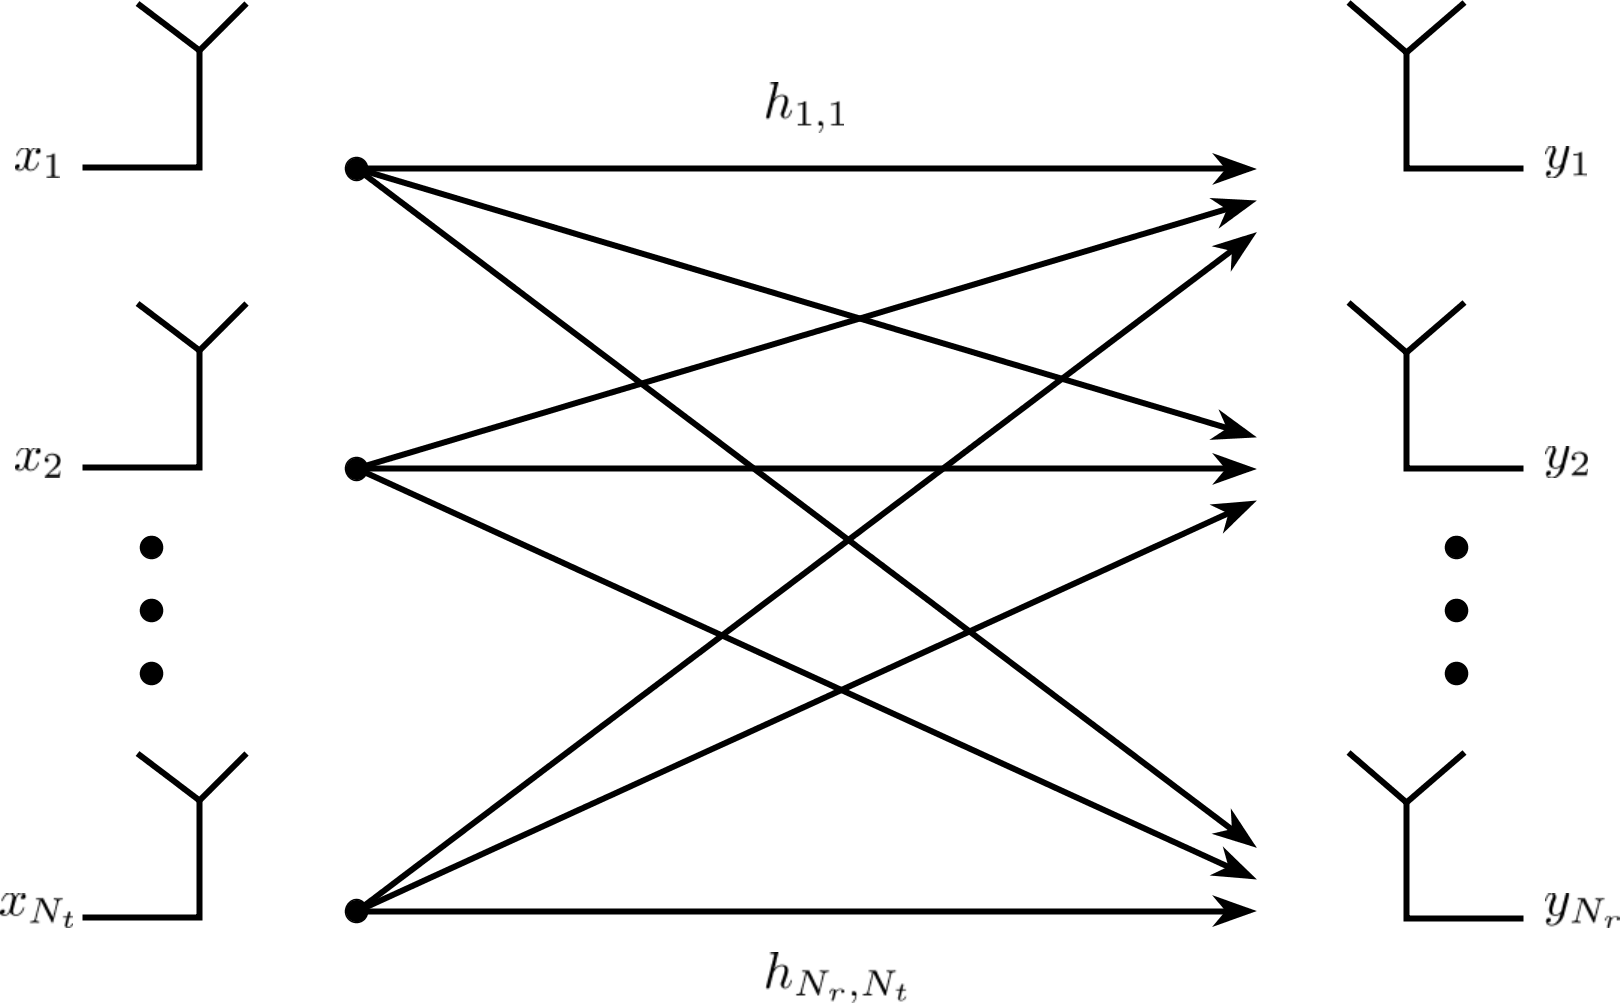
\includegraphics[width=\linewidth]{images/MIMO_Illustration.jpg}
        \caption{MIMO channel model}
        \label{fig:MIMOChannel}
    \end{center}
\end{figure}

\begin{equation}
    \hat{x} = Wy
\end{equation}

Once the channels propogation effects have been calculated each symbol has to be equalized to compensate the distortion effect caused by the dispersive channel. In the case of a MIMO channel there are 3 main algorithms which are as follows

\subsection{Maximum Ratio Combiner}\label{ssec:Simple}

\begin{equation}
    W_{MRC} = C\hat{H}^H
\end{equation}
where $C$ is a diagonal matrix with 

\begin{equation}
    C_{k,k} = \left ( {\sum_{m}} \left | H_{m,k} \right |^2 \right )^{-1}
\end{equation}

and can be considered as a normaliser for the columns of the matrix $H$.

\subsection{Zero Forcing}\label{ssec:ZF}

\begin{equation}
    W_{ZF} = (\hat{H}^H\hat{H})^{-1}\hat{H}^H
\end{equation}

Zero forcing is an algorithm that is avoided although given its simplicity, the reason being that the noise can be amplified in the case of a low SNR situation. Hence in practice this algoritm is avoided. The implimentation is a Least squares estimate of the vector $\hat{x}$.

\subsection{MMSE}\label{ssec:MMSE}

\begin{equation}
    W_{MMSE} = (\hat{H}^H\hat{H}+\sigma^{2}I)^{-1}\hat{H}^H
\end{equation}

where $\sigma$ is the inverse SNR.

MMSE algorithm performs the best under all situations. For high SNR scenarios it converges to an ZF algorithm and for a low SNR situation it converges to the MRC algorithm.

%\subsection{No Equalisation}\label{ssec:NoEq}
%\begin{equation}
%    W_{NoEq} = I
%\end{equation}
%
%This equalisation means that 


\chapter{Potential Hardware Setups}
\label{ch:PotenHWSetup}

Measurements of MIMO channel can be achieved in multiple methods. This chapter discusses some of the potential approaches which were implemented and elaborates each of their advantages and disadvantages.

\section{Software Defined Radios USRP}\label{sec:USRP}

USRP is a Software Defined Radio (SDR) designed by National Instruments that enables quick prototyping of different wireless applications. It is aimed at anyone from hobbists, research labs, universities, etc... or anyone interested in evaluating custom algorithms. The SDR used here is a USRP2940 specifications of which are described in Table \ref{tb:USRP}

\begin{table}[H]
    \begin{center}
        \begin{tabular}{|l|c|}
        \hline
            Model                   & USRP2940          \\ \hline
            Baseband Bandwidth      & 40MHz             \\ \hline
            RF-Operating Frequency  & 50MHz-2200MHz     \\ \hline
            FPGA                    & Kintex-7 410T     \\ \hline
            No of Transmitters      & 2                 \\ \hline
            No of Receivers         & 2                 \\ \hline
            Connectivity            & MXIe, Ethernet    \\ \hline
            Oscillator              & Internal Crystal  \\ \hline
            ADC/DAC                 & 14 (For Rx)/16 (For Tx) bit         \\ \hline
            Frequency Accuracy      & 2.5 ppm           \\ \hline
            Maximum Power Output    & 20dBm             \\ \hline
        \end{tabular}
    \end{center}
    \caption{USRP SDR Product details}
    \label{tb:USRP}
\end{table}

%\begin{table}[H]
%    \begin{center}
%        \begin{tabular}{|c|c|}
%            \hline
%            Parameter & Value \\ \hline
%            RBW & 20kHz \\ \hline
%            VBW & 50kHz \\ \hline
%            SWP Time & 50ms  \\ 
%            \hline
%        \end{tabular}
%    \end{center}
%    \caption{Spectrum analyser settings for the transmit power tests}
%    \label{}
%\end{table}

\section{MIMO Application Framework}\label{sec:MIMOAFW}
\section{LTE Application Framework}\label{sec:LTEAFW}



%\begin{figure}[!htb]
%    \centering
%    \includegraphics[width=7cm]{../ReportImages/TxPwrSetup.png}
%    \caption{Setup for measuring the transmit power}%
%    \label{fig:TxPwrSetup}%
%\end{figure}


\chapter{Experimantal Setup}
\label{ch:ExSetup}

Chapter \ref{ch:PotenHWSetup} discussed the possible options to implement a MIMO setup. The first option (section \ref{sec:USRP}) was not viable due to technical limitations as it is described in \ref{sec:USRPSync}.

The second option (section \ref{sec:MIMOAFW}) was financially unfeasible as the additional hardware for the synchronisation was to cost over €80.000

\section{LTE Application Framework}\label{sec:LTEAFW}
The 
\section{Application Example}\label{sec:AppEx}


\chapter{Results}
\label{ch:results}

Over the course of the internship many different parameters had to be determined and set up for the final demo. This chapters documents the results of all the experiments performed as well as the final demo of the working setup.

\section{Over-the-air User Data Transmission}\label{sec:OTADataTrans}

Following the data transmission through over the air using LTE AFW, benchmarks were run to check the loss of data over the wireless medium. Data loss tests were profiled using \textit{iperf}, a software used to profile UDP traffic.

A server and client of the version of the iperf application was used to test the wireless interface. Where the data was produced by the client on UDP port \texttt{50000} and received on the localhost \texttt{127.0.0.1} on UDP port \texttt{60000} once a SISO and MIMO Tx-Rx wireless interface was setup for the respective tests. The version of iperf used is shown below.

\begin{lstlisting}[style=DOS]
iperf version 2.0.9 (1 June 2016) pthreads
\end{lstlisting}

The command used to start up a Client is shown below.
\begin{lstlisting}[style=DOS]
iperf.exe -c 127.0.0.1 -u -i 1 -b 10M -t 10 -p 50000
\end{lstlisting}

The command used to start up a server is shown below.
\begin{lstlisting}[style=DOS]
iperf.exe -s -u -B 127.0.0.1 -i 1 -p 60000
\end{lstlisting}

\subsection{SISO}\label{ssec:SISOOTA}

A SISO communications channel was setup with the Tx and Rx settings as mentioned in Table \ref{tab:TXUSRPParam} and \ref{tab:RXUSRPParam} using the LTE AFW template. On conducting UDP data flow tests, it was observed that there were no packet drops with a UDP data block loss rate of $0\%$.

As a next step a short video clip was fed into the UDP stream of the transmitter and received with no video and audio frame drops at all. The demo video can be seen here \cite{}.

\subsection{MIMO}\label{ssec:MIMOOTA}

In the second test a MIMO communications channel was setup with the Tx and Rx settings as mentioned in Table \ref{tab:TXUSRPParam} and \ref{tab:RXUSRPParam} using the LTE MIMO AFW 2x2 extention software. On conducting UDP data flow tests, it was observed that there were large packet losses with a UDP data block loss rate of around $25\%$. Below is an output of the server client iperf application.


\begin{lstlisting}[style=DOS]
Microsoft Windows [Version 10.0.18363.1016]
(c) 2019 Microsoft Corporation. Alle Rechte vorbehalten.

C:\Users\ge69mog>cd Downloads\iperf-2.0.9-win64\iperf-2.0.9-win64

C:\Users\ge69mog\Downloads\iperf-2.0.9-win64\iperf-2.0.9-win64>iperf.exe -s -u
-B 127.0.0.1 -i 1 -p 60000
------------------------------------------------------------
Server listening on UDP port 60000
Binding to local address 127.0.0.1
Receiving 1470 byte datagrams
UDP buffer size:  208 KByte (default)
------------------------------------------------------------
[  3] local 127.0.0.1 port 60000 connected with 127.0.0.1 port 49721
[ ID] Interval       Transfer     Bandwidth        Jitter   Lost/Total Datagrams
[  3]  0.0- 1.0 sec   996 KBytes  8.16 Mbits/sec   2.017 ms  166/  860 ((*@\textcolor{red}{19\%}@*))
[  3] 0.00-1.00 sec  50 datagrams received out-of-order
[  3]  1.0- 2.0 sec   904 KBytes  7.41 Mbits/sec   2.426 ms  227/  857 ((*@\textcolor{red}{26\%}@*))
[  3] 1.00-2.00 sec  70 datagrams received out-of-order
[  3]  2.0- 3.0 sec   902 KBytes  7.39 Mbits/sec   2.148 ms  219/  847 ((*@\textcolor{red}{26\%}@*))
[  3] 2.00-3.00 sec  61 datagrams received out-of-order
[  3]  3.0- 4.0 sec   916 KBytes  7.50 Mbits/sec   1.904 ms  222/  860 ((*@\textcolor{red}{26\%}@*))
[  3] 3.00-4.00 sec  69 datagrams received out-of-order
[  3]  4.0- 5.0 sec   871 KBytes  7.14 Mbits/sec   4.137 ms  206/  813 ((*@\textcolor{red}{25\%}@*))
[  3] 4.00-5.00 sec  56 datagrams received out-of-order
[  3]  5.0- 6.0 sec   953 KBytes  7.81 Mbits/sec   4.710 ms  226/  890 ((*@\textcolor{red}{25\%}@*))
[  3] 5.00-6.00 sec  86 datagrams received out-of-order
[  3]  6.0- 7.0 sec   828 KBytes  6.79 Mbits/sec   2.786 ms  253/  830 ((*@\textcolor{red}{30\%}@*))
[  3] 6.00-7.00 sec  84 datagrams received out-of-order
[  3]  7.0- 8.0 sec   843 KBytes  6.90 Mbits/sec   4.467 ms  250/  837 ((*@\textcolor{red}{30\%}@*))
[  3] 7.00-8.00 sec  90 datagrams received out-of-order
[  3]  8.0- 9.0 sec   970 KBytes  7.95 Mbits/sec   1.648 ms  200/  876 ((*@\textcolor{red}{23\%}@*))
[  3] 8.00-9.00 sec  61 datagrams received out-of-order
[  3]  0.0-10.0 sec  8.86 MBytes  7.43 Mbits/sec   2.888 ms 2183/ 8505 ((*@\textcolor{red}{26\%}@*))
[  3] 0.00-10.00 sec  689 datagrams received out-of-order

\end{lstlisting}

The same short video clip that was used in the SISO case was fed into the UDP stream of the transmitter and received with large distortion and missing several frames of the video and audio.

It was inferred as a result of the tests that this loss stems from the CPU overhead in processing 2 simultaneous UDP streams of data, or the handling of UDP data by the LTE AFW 2x2 MIMO extension application.

\section{CRS Data Transmission}\label{sec:CRSDataVisualisation}
As seen from the results of the previous section, the data loss in the user data sent via UDP was not a feasible option for the purposes of this experiment as data had to be received any losses. As a result, it was decided to use the CRS symbols as sent and received data pairs. This was done by utilising $h_{11}$ and $h_{22}$ as received unequalized symbols. Figure \ref{fig:XYPairsCRS} shows that the $h_{11}$ channel coefficients correspond to the 
CRS signal arranged in the grid for antenna port 0 and $h_{22}$ channel coefficientes correspond to the CRS signals arranged in the grid for antenna port 1. Since this data is processed in the FPGA fabric, it is real time and there is no lost CRS symbol being forwarded to the Host.

The sending pattern is fixed as it is defined in the standard and the corresponding received CRS symbols can be obtained from the $h_{11}$ (Channel estimate of channel between transmit antenna 1 and receive antenna 1) and $h_{22}$ (Channel estimate of channel between transmit antenna 2 and receive antenna 2) signals respectively.

A sequence of $8342$ time CRS symbols were recorded over the complete 20 \si{\mega\hertz} bandwidth of the LTE spectrum. This corresponds to 200 subcarriers which bear the reference pilot symbols. Hence a matrix of size $200\times8342$ was generated for the training of the inverse neural network.

\section{Inverse Neural Network Detection}\label{sec:INNDet}

Following the generation of experimental data, one particular subcarrier was chosen as training data set ,i.e. one row of the above mentioned Matrix. The first CRS subcarrier was chosen

And the related wideband SINR for each time symbol was also recorded, this was the second input needed by the training network (as mentioned in Section \ref{ssec:SINR}).

\subsection{INN Constellation}\label{ssec:INNConstellation}

Figure \ref{fig:INNxn} shows the input CRS signals added with random received noise wideband noise for the different time instants. If the signal was added with the wideband noise, then there are infinite mapping possibilties between the input and the output, as one point could map to a set of infinite continuous point on the output. And this would be a NP Hard problem. To avoid this the approach of adding the wideband noise was taken to create a clusters of inputs and corresponding outputs to form a bijective mapping. This was computable and could be used by the network. $x_1$ and $x_2$ are the real parts of the CRS signals for antenna port 0 and antenna port 1 respectively. These are QPSK signals that can take the possible values  $\pm \frac{1}{\sqrt{2}} \pm j \frac{1}{\sqrt{2}}$. Just using the real parts we have 4 possibilites where $x_1$ and $x_2$ can assume the value of $\pm \frac{1}{\sqrt{2}}$ each. But due to the inherent structure of the CRS symbols in the LTE standard, only one of the possible above combinations is found namely, +$\frac{1}{\sqrt{2}}$,-$\frac{1}{\sqrt{2}}$
%\begin{equation} \label{eq:QPSKSymbols} 
%\end{equation}

\begin{figure}[!htb]
    \centering
    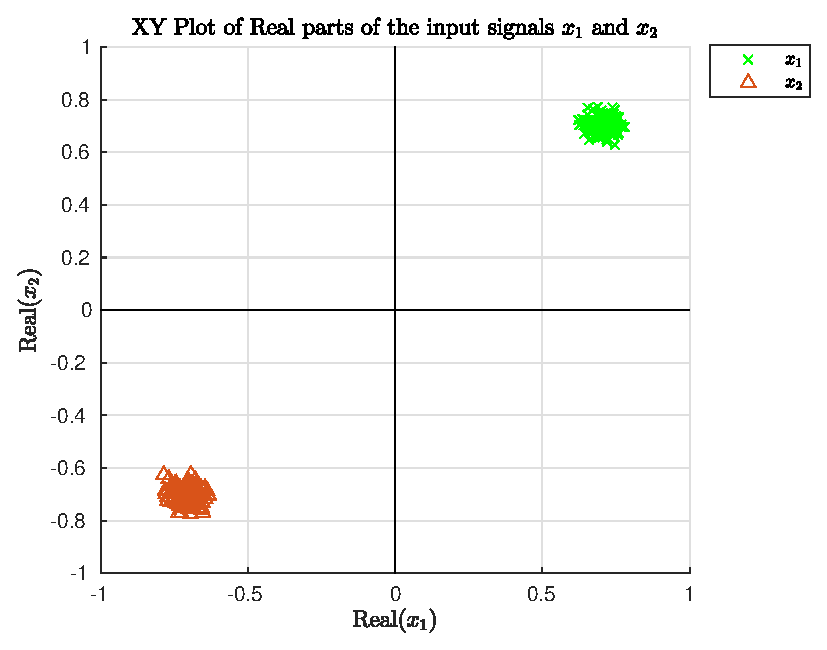
\includegraphics[width=\linewidth]{images/INNxn.eps}
    \caption{XY plot of the real parts of the input signals $x_1$ and $x_2$ with noise}
    \label{fig:INNxn}
\end{figure}

The Figure \ref{fig:INNyn} shows the received channel estimates $y_1 = h_{11}$ and $y_2 = h_{22}$. The phase shift in the various samples, represents the channel distortion effects.

\begin{figure}[!htb]
    \centering
    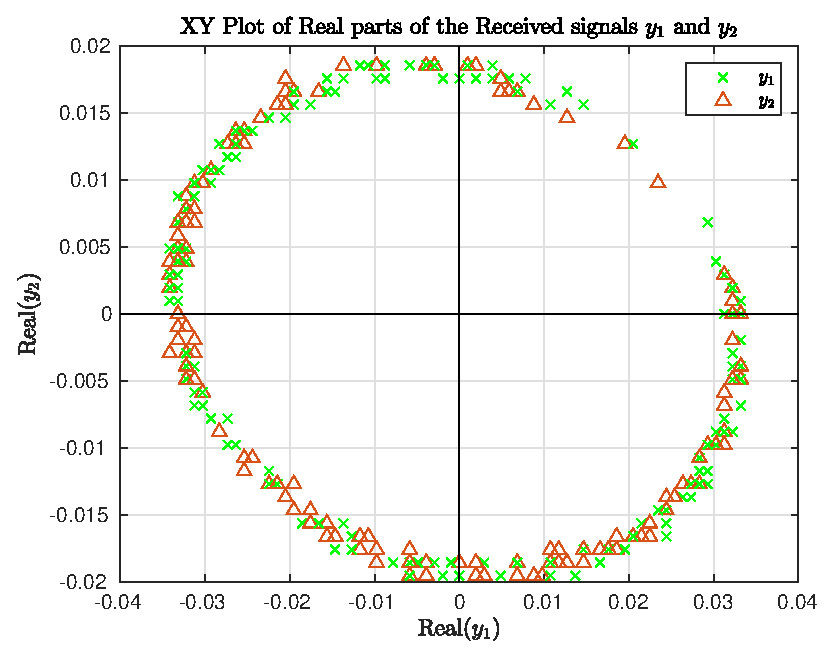
\includegraphics[width=\linewidth]{images/INNyn.eps}
    \caption{XY plot of the real parts of the received signals $y_1$ and $y_2$}
    \label{fig:INNyn}
\end{figure}

\begin{figure}[!htb]
    \centering
    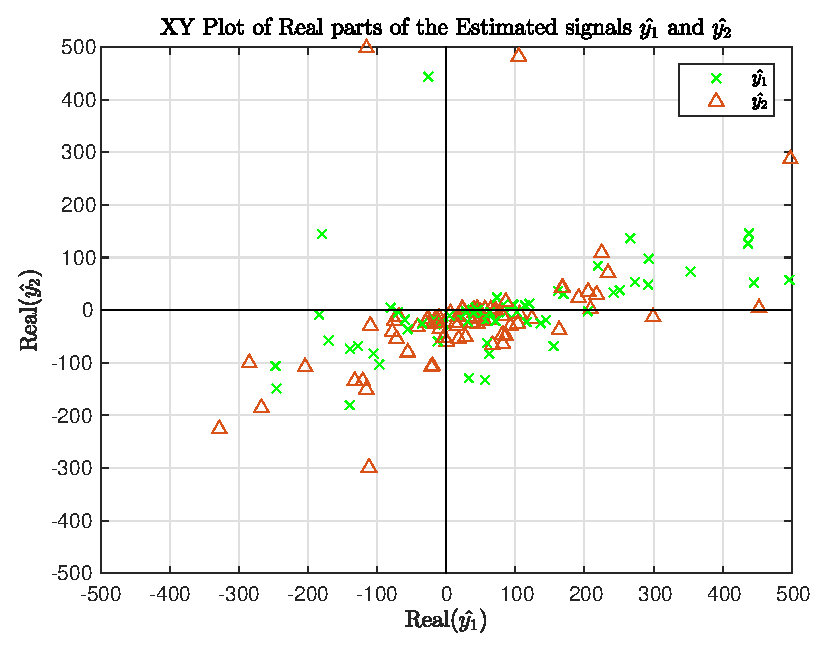
\includegraphics[width=\linewidth]{images/INNResult.eps}
    \caption{XY plot of the real parts of the INN Estimated signals $\hat{y_1}$ and $\hat{y_2}$ }
    \label{fig:INNyResult}
\end{figure}

\chapter{Conclusion and Outlook}\label{ch:conOutlook}

\section{FPGA File Port}\label{sec:FPGAChange}
Currently the FPGA Hardware design is where all the data is being received from the RF Front end and processed. This is a pre compiled bit file delivered by NI to work with their version of the LTE AFW Software. To adapt the design to suit the needs of the current research, the FPGA bit file has to be ported to suit our design 

%TODO add photos of the missing dependencies

\section{Experiment with structured Channel}\label{sec:StrucChannel}



%\chapter{Example with Citations}
%\blindtext
%
%\section{Citation and Equation}
%If we write a floating point definition without suffixes$\mathrm{suffixes}\operatorname{suffixes}$ as in $y = \sin(x)$ sin(x), we obtain inline math symbols~\cite{Aldroubi01,Bazaraa06,WeStSh06}.
%\begin{equation}
%\prod_{j=1}^J\sum_{i=1}^\infty \int_{-\infty}^\zeta e^{\xi^2/\nu}d\xi \int_{S^1} \mathcal{R}f_i^j(\omega) d\omega
%\end{equation}
%\begin{equation}
%\left(\frac{\sin(x)}{\pi x} <\leq=\geq>|\|\sim+-\pm \| z^Hz\|\right)\quad \forall \zeta \in R
%\end{equation}%
%
%\blindtext[8]
%
%\section{This is a Section}
%\blindtext[1]
%
%\subsection{This is a Subsection}
%\blindtext[1]
%
%\subsubsection{This is a Subsubsection}
%\blindtext[1]
%
%\paragraph{This is a Paragraph}
%\blindtext[1]
%
%\subparagraph{This is a Subparagraph}
%\blindtext[1]
%
%
%\chapter{Check Text Height}
%\blindtext[40]
%
%\blindmathtrue
%\Blinddocument
%\blinddocument


%--------------------------------------------------------------------------------
% ** Appendix
%
\appendix
\chapter{Schematic Octoclock}
\label{ch:HWSchOctoClock}

%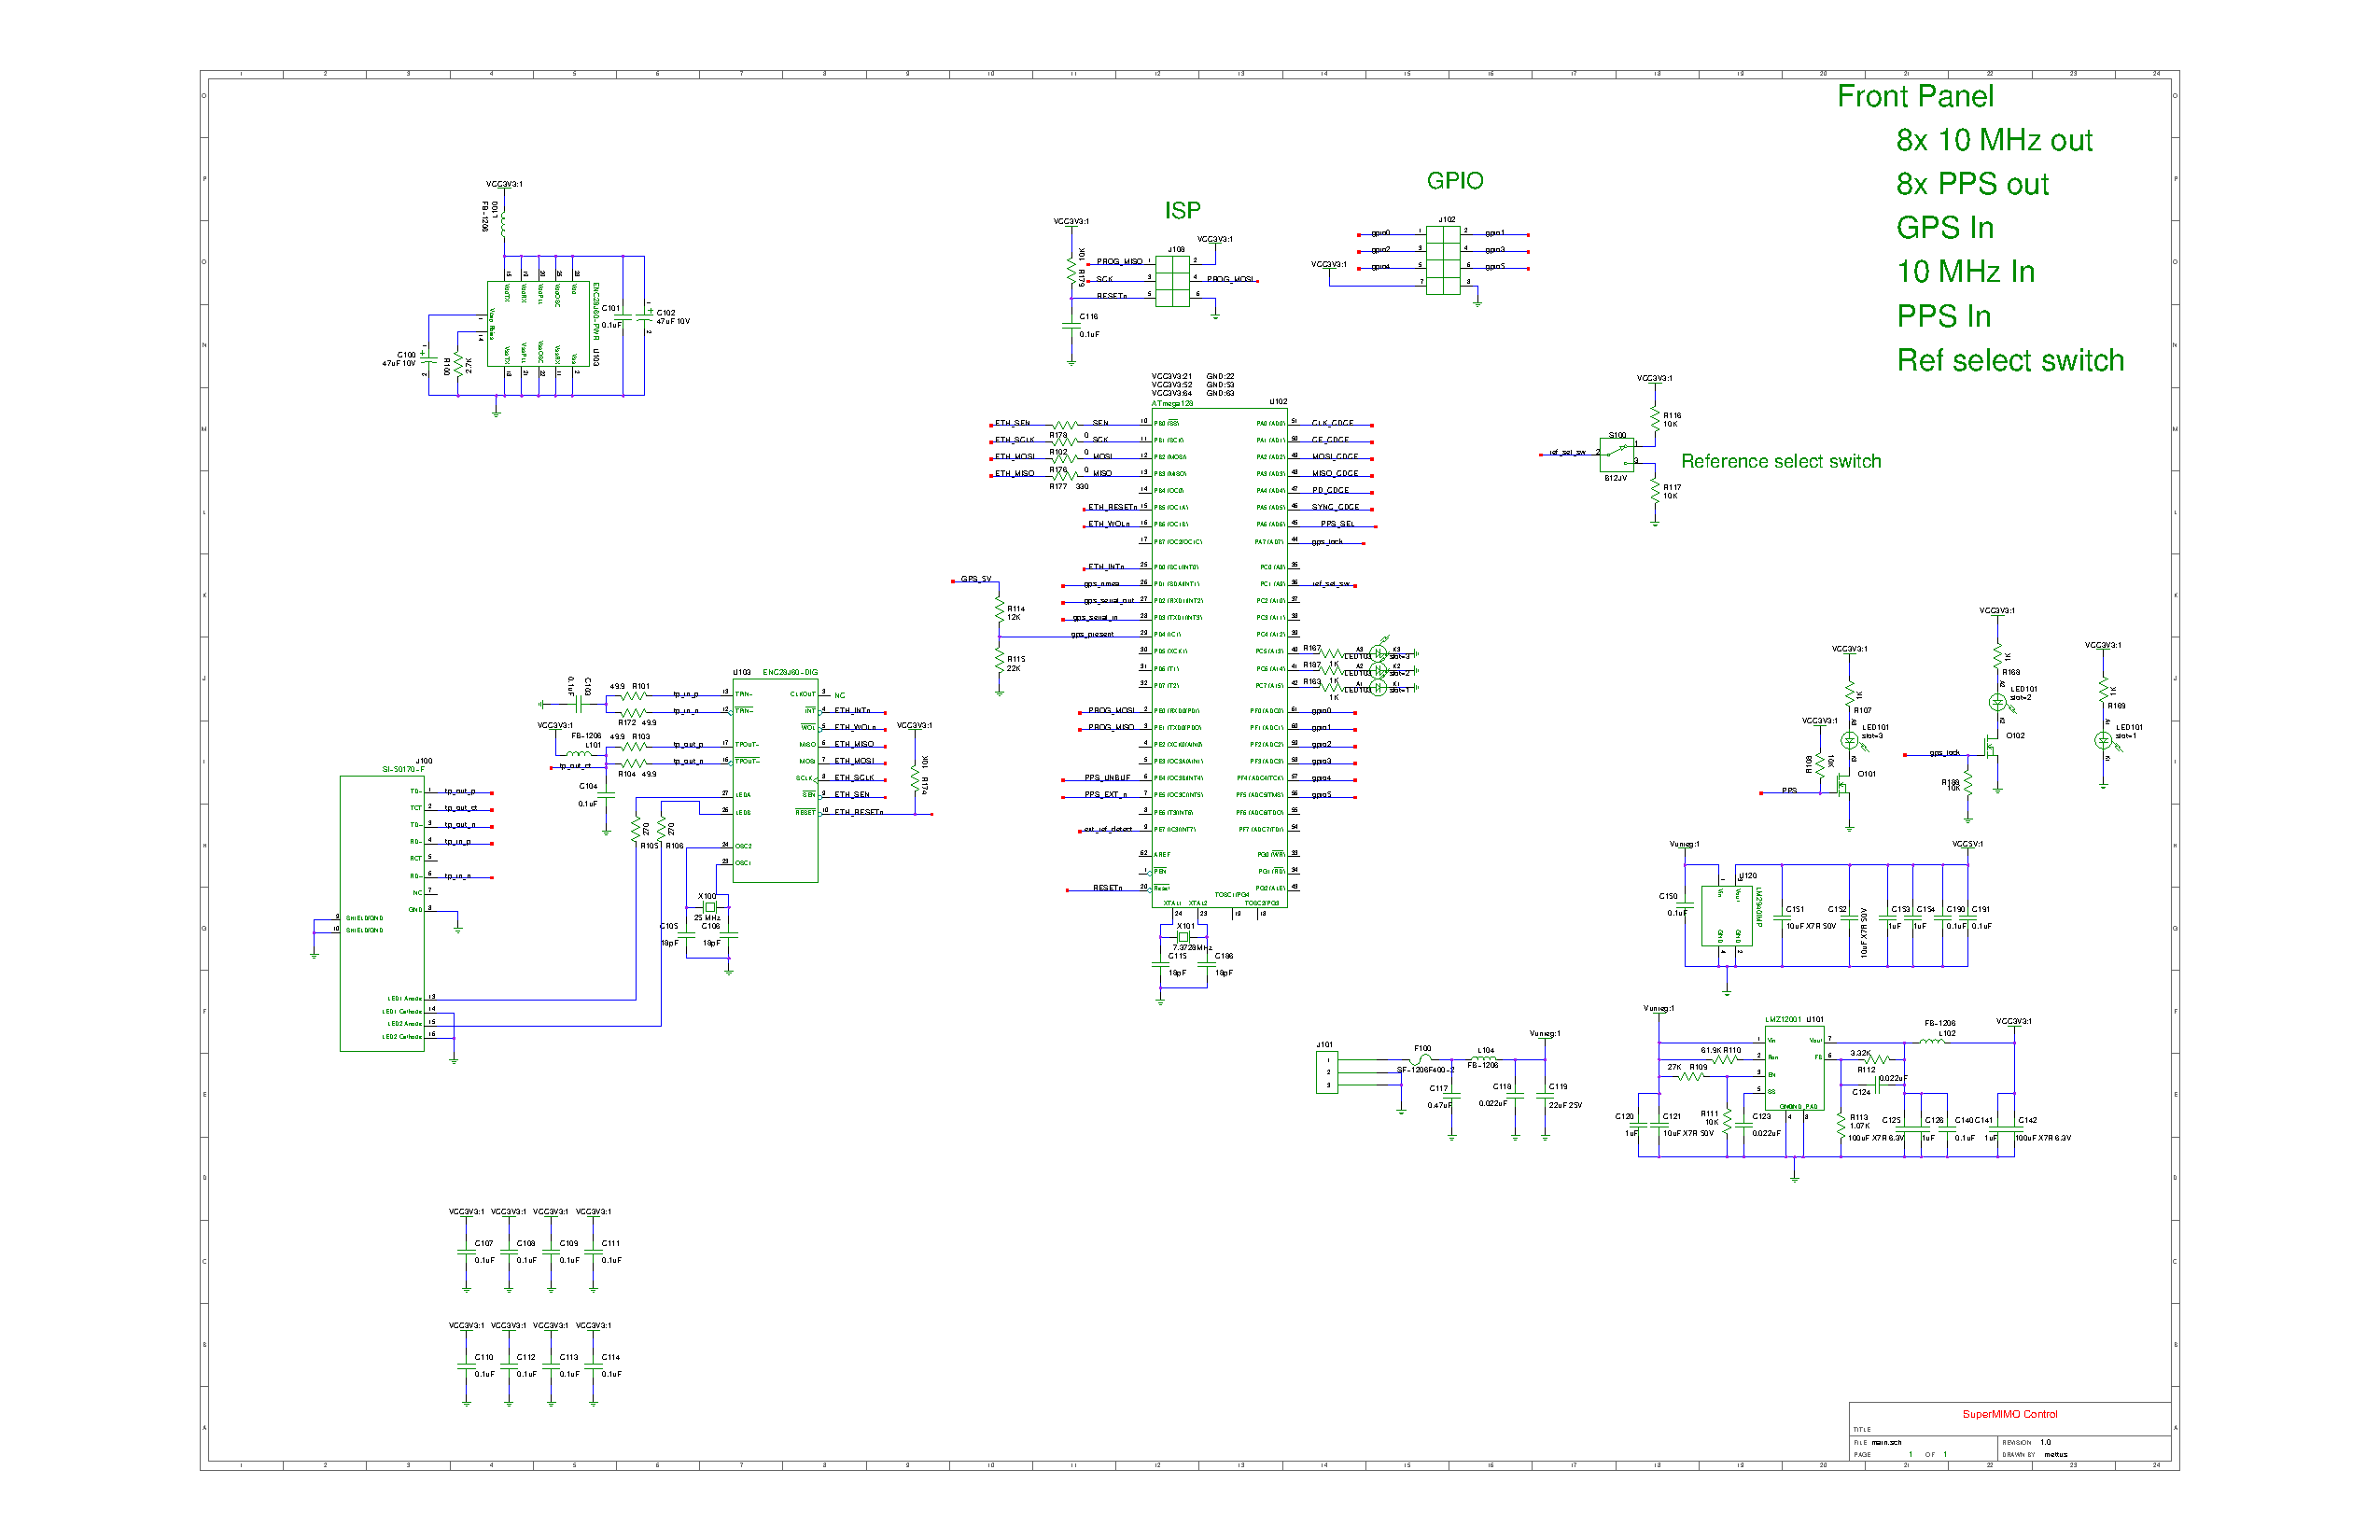
\includepdf[pages=-]{images/OctoclockSchematics/octoclock.pdf} between \begin{document} and \end{document}

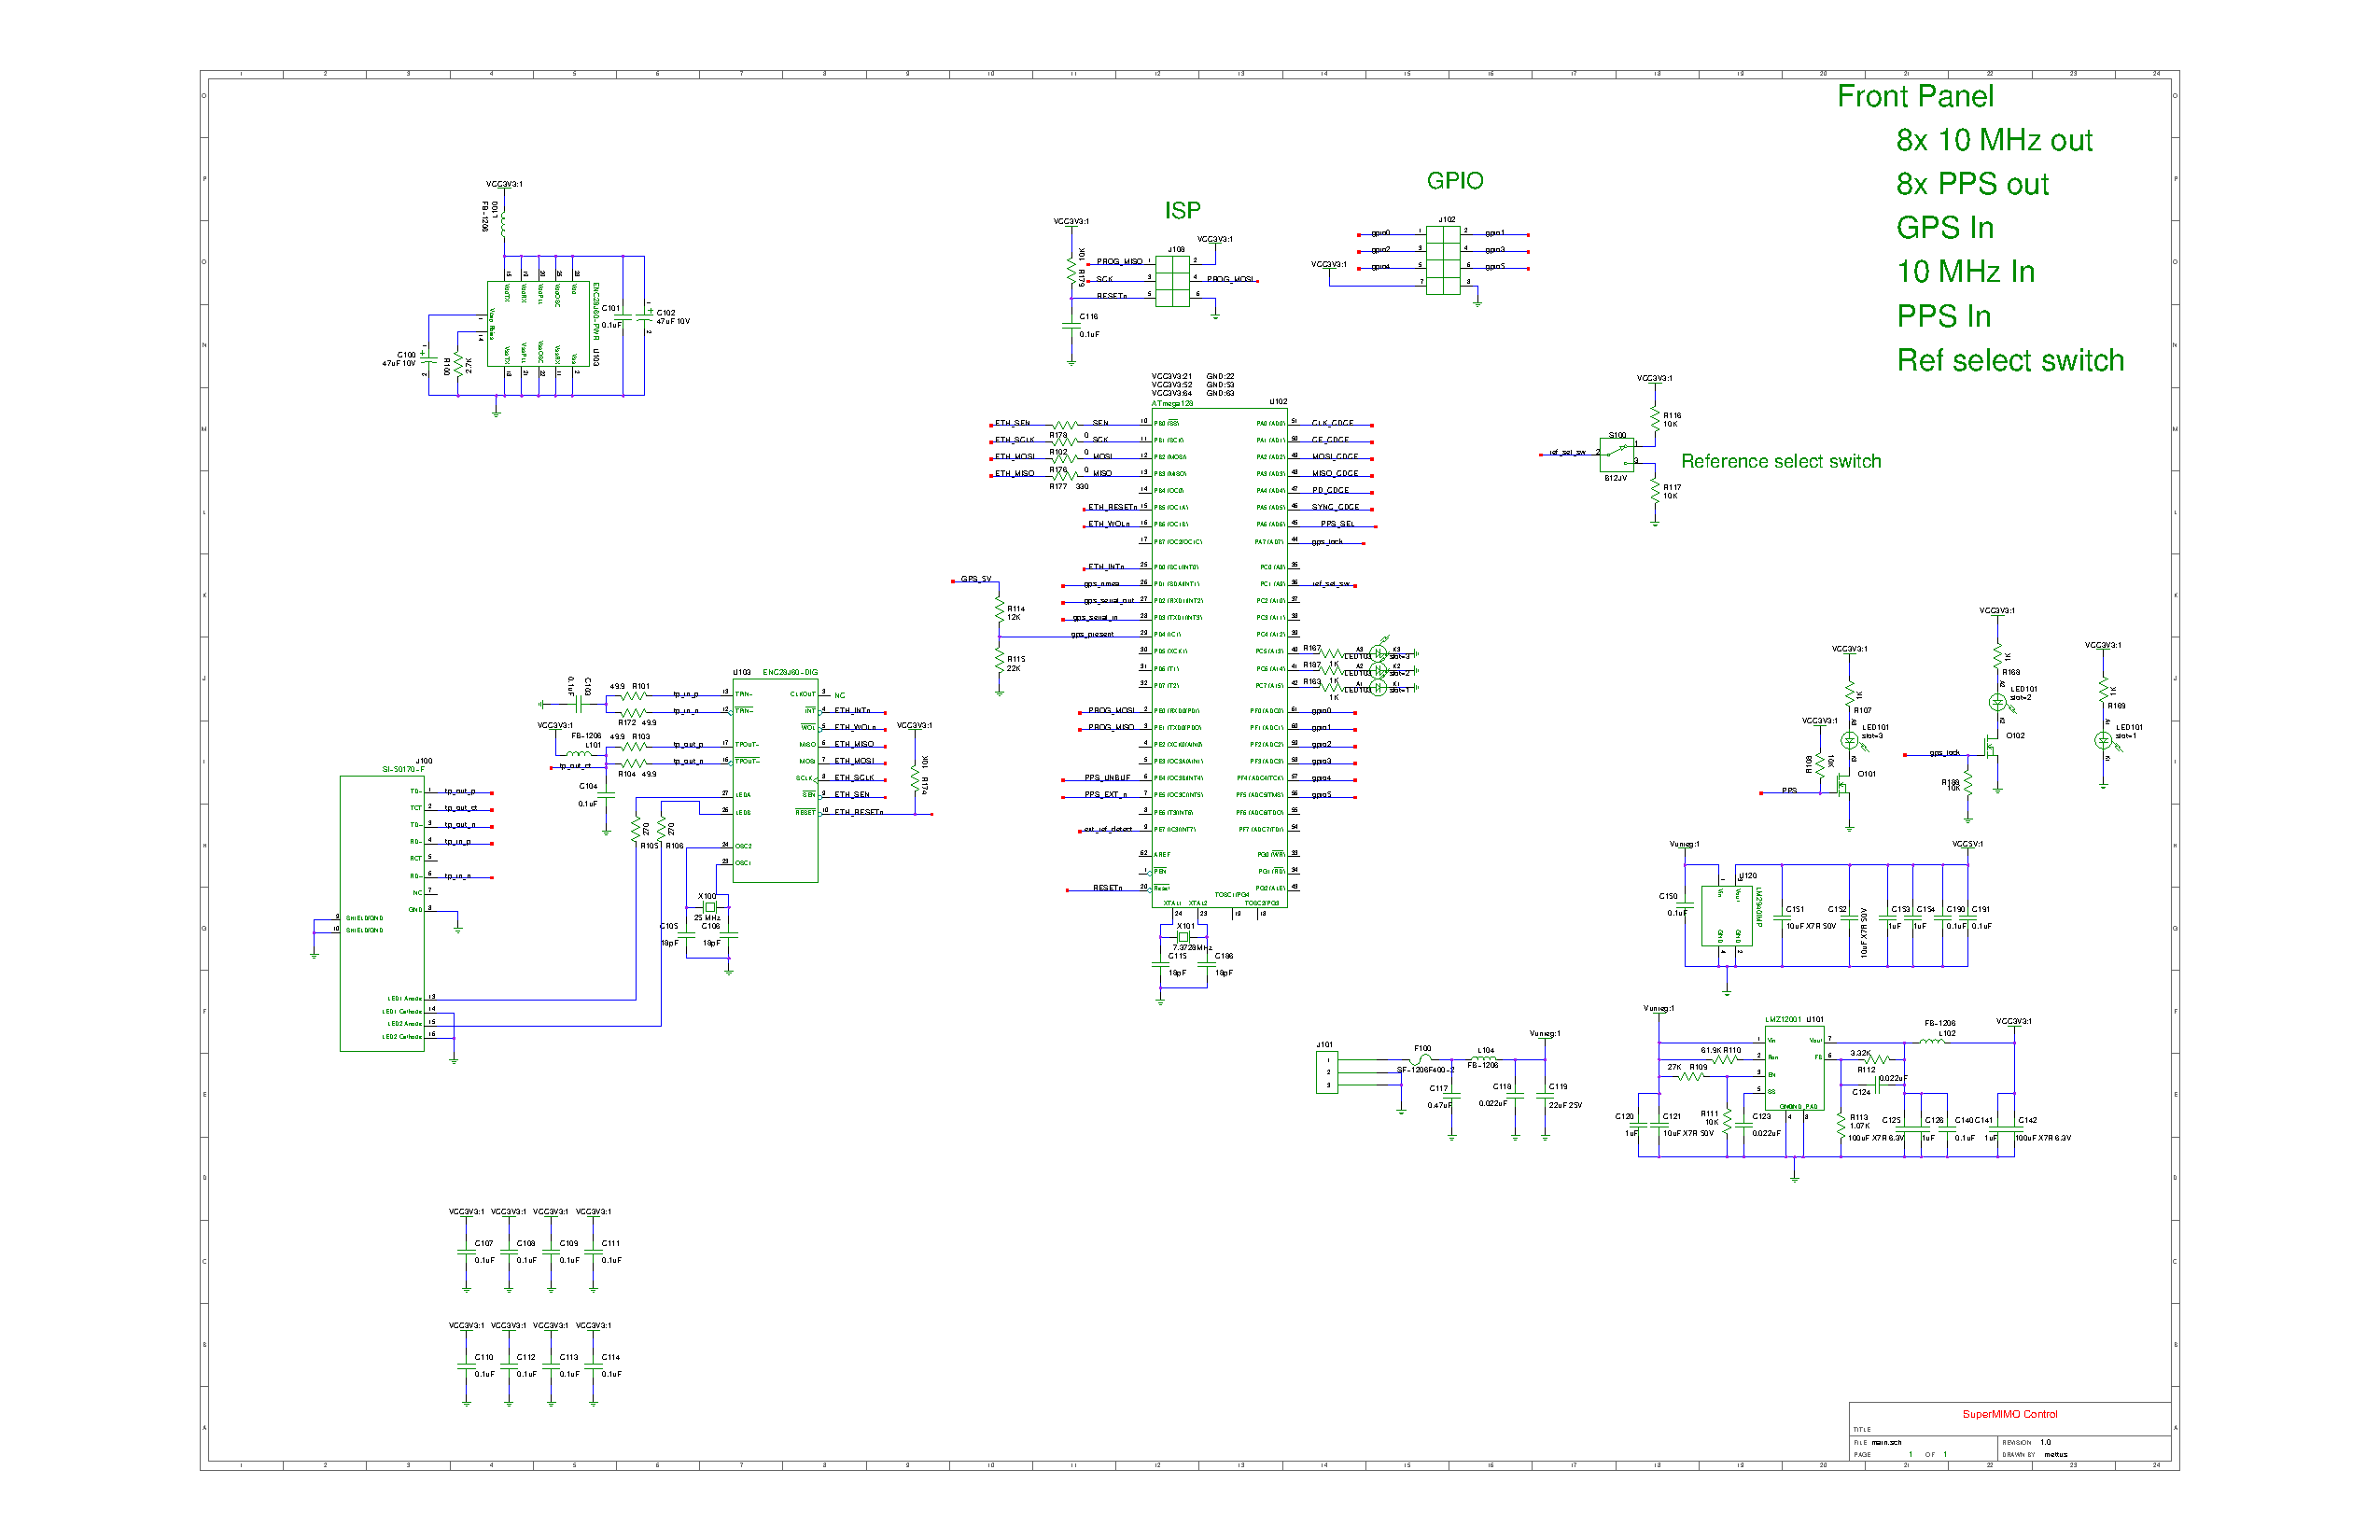
\includepdf[pages={1,2}, angle=-90]{images/OctoclockSchematics/octoclock.pdf}

%\begin{figure}[!htb]
%    \centering
%    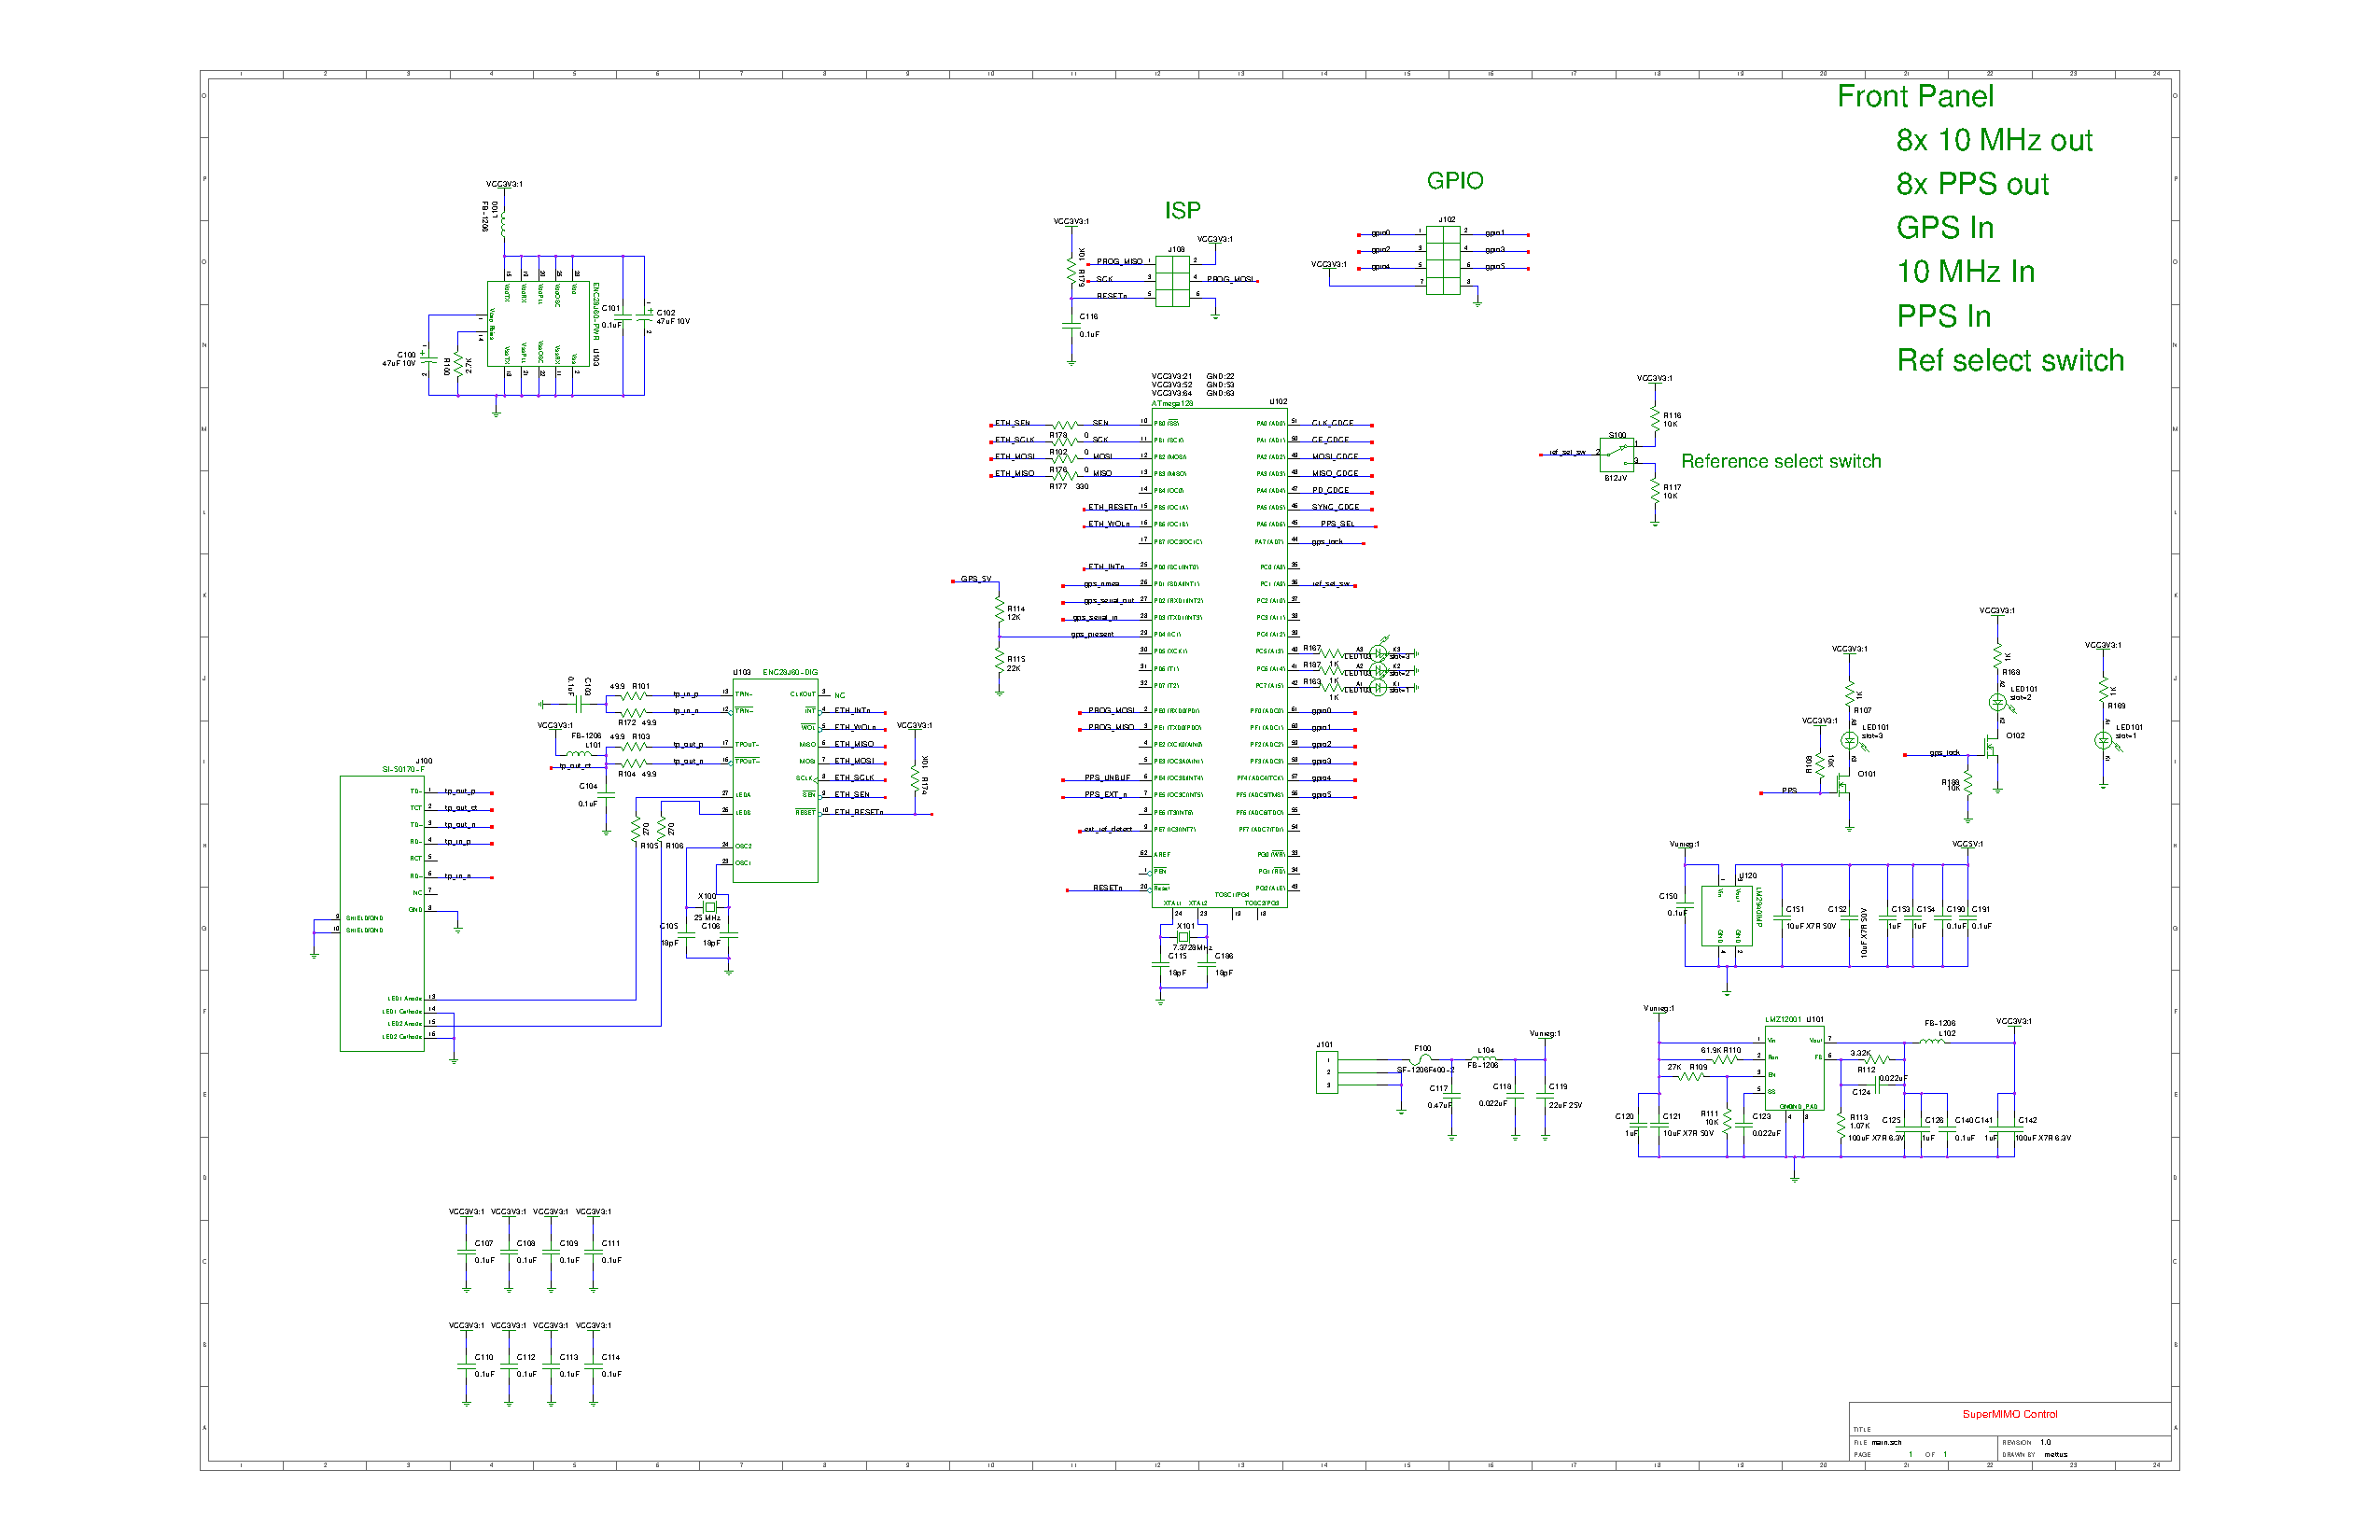
\includegraphics{images/OctoclockSchematics/octoclock.pdf}
%    \caption{Schematics for the Octoclock Clock Distribution}%
%    \label{fig:OctClkSch}%
%\end{figure}

\chapter{Troubleshooting}\label{ch:troubleshooting}
\section{Boot Order} \label{sec:BootOrder}
\section{Synchronisation of the USRPs} \label{sec:USRPSync}



\cleardoublepage
% \bibliographystyle{unsrt}
%--------------------------------------------------------------------------------
% ** References 
\bibliographystyle{IEEEtran}
\refstepcounter{chapter}
\addcontentsline{toc}{chapter}{\bibname}
\bibliography{bibfile}

% \cleardoublepage
% \refstepcounter{chapter}
% \addcontentsline{toc}{chapter}{\indexname}
% \printindex
% \end{comment}
\end{document}
